\documentclass[11pt, oneside]{article}   	
\usepackage[margin = 1 in]{geometry}                		
\geometry{letterpaper}                   		
%\usepackage[parfill]{parskip}    %Begin paragraphs with an empty line rather than an indent
\usepackage{graphicx}				
\usepackage{setspace}								
\usepackage{amssymb}
\doublespacing
%\geometry{footnotesep=2\baselineskip}
\usepackage{longtable}
\usepackage{caption} %Put caption* in a table to remove the enumeration
\usepackage{rotating} % To rotate the reviewer table
\usepackage{natbib}   %activates bibliography
\usepackage [english]{babel} %something for bibliography
\usepackage{verbatim} %to be able to use \begin{comment}
\usepackage{booktabs}
\usepackage{array}
\usepackage{float} 
\usepackage{lscape} %allows for one page to be landscape


\begin{document}


\begin{comment}
5/28 TO-DO:
Check to see if matches: 
	Table references to tables --DONE
	Section references to sections --DONE
Make sure Figures 1,2 come before table 1 in text. if not, change order in "full_tables.tex" --DONE
put in more appropriate stats in data section for in-city comparison
rewrite conclusion --DONE

Options for first sentence of abstract:
\begin{enumerate}
\item The extent of discrimination on Airbnb, especially against hosts, remains poorly researched. 
\item Despite well-publicized efforts by Airbnb to address discrimination on its platform, the discrimination against hosts remains poorly measured by economists. 
\item Even though discrimination against hosts on Airbnb carries serious economic consequences for agents, the issue has remained poorly researched. 
\item Measuring discrimination is challenging because in the absence of an experiment, it requires controlling for an extensive set of covariates. 
\item Little research has been done on the extent of discrimination against hosts on Airbnb because of data restrictions, and difficulty of setting up an experiment. 
\item This paper leverages the recent rise of sharing economies and the data and standardization their platforms provide to credibly measure discrimination against minority landlords
\item There is little evidence that these price disparities are due to minority hosts choosing to price their listings lower because of differences in their marginal cost, or offering their listing up for rent for shorter periods of time, than white hosts. I also find little evidence that this effect is due to minority hosts owning listings of worse quality.(LAST SENTENCE OF FORMER ABSTRACT)  
\end{enumerate}
\end{comment}


\title{Measuring Discrimination: The Impact of Host Race and Gender on Earnings from Airbnb\footnote
	{I thank Steven D. Levitt for valuable advice. Kirthi Bellamkonda, Jacob Dorn, Michal Dzitko, Sonia Jaffe, Ezra Karger, Sylvia Klosin, Victor Lima, and Kotaro Yoshida provided excellent feedback and comments. Mahathi Ayyagari, Fong Chai, Joseph Day, Melody Jih, Spencer Kang, Cristian Raygoza, Tony Song, Lydia Sum, Putter Thepkanjana, and Leah Umanskiy provided research assistance. All remaining errors are my own. Data was provided by InsideAirbnb.com, founded and maintained by Murray Cox. Airbnb was not consulted in this research. Sentiment analysis would not be possible without Sentimentr and coding by Ben Chaimberg.}}
\author{Anya Marchenko}
\maketitle


\begin{abstract}
Measuring discrimination is challenging because in the absence of an experiment, the presence of unobservables confounds estimates of discrimination. This paper leverages the recent rise of sharing economies and the data and standardization their platforms provide to credibly measure discrimination against minority landlords on Airbnb. Earlier research has attempted to measure discrimination against New York City hosts, but was limited by a small sample size and no credible way to tease out the effects of discrimination. I address this issue by using a previously unexploited dataset from a large webscrape of the Airbnb website. Controlling for a large set of covariates, I estimate that black hosts earn \$5 - 7 less per night, and Asian hosts \$6 - 9 less per night (depending on the sex of the host) than white hosts who post a similar type of listing. Crucially, I have a measure of quantity demanded of hosts' listings, which allows me estimate whether a demand or supply shift is responsible for the price disparity. I estimate that quantity demanded is lower for minority hosts, consistent with discrimination. 
\end{abstract}


\doublespacing
\section{Introduction}


African-Americans experience pervasively worse outcomes in the housing market as a result of historic and current racial discrimination \citep{krysan}. Even after the gains during the Civil Rights Era, such as the landmark Fair Housing Act of 1968, discrimination in the housing market is widely documented by social scientists. African-American renters are told that there are 30\% fewer available housing units than white renters \citep{yinger1}. African-American families face higher barriers when raising capital to purchase a home \citep{pope}. E-mails sent to landlords from home-seekers with typical African-American names receive lower response rates than emails sent by those with names commonly associated with whites \citep{hanson}.%
	\footnote{Some studies have found evidence that discrimination in rental markets is statistical in nature (that is, landlords use race as a proxy for income). For African-Americans who imply that they are of a higher social class when applying for an apartment, discrimination is virtually not present \citep{hanson}.}

%\citep{yinger1}
%Landlords renting out apartments discriminate both because of their own prejudice and in response to the prejudice of their white renters \citep{ondrich}.

Economists have primarily studied discrimination against African-American tenants. There is little research on the other side of the market - when African-Americans are supplying, rather than demanding, housing. Because property ownership cannot be randomized, it is difficult to disentangle true discrimination from systematic differences in the housing owned by African-Americans and white landlords.%
	\footnote{One would also expect black landlords to fare worse than white landlords in this area as well. Properties owned by African-Americans tend to be less expensive than those owned by white Americans. The average black household still has less mean wealth than a white household \citep{oliver}. Even middle-class black and Hispanic households still live in neighborhoods with median incomes similar to those of very poor white neighborhoods \citep{reardon}.} 
Some studies have found evidence that African-American homeowners are more likely to be targeted by subprime loans \citep{foreclosure} or pay more than whites for similar housing \citep{bayer} \citep{myers}, but few studies have a credible identification strategy to separate discrimination from correlated observables. 

%Some studies have found correlatory evidence of discrimination against African-American homeowners, but none have a credible mechanism to identified disrimination from other factors. For instance, the spike in subprime lending and the ensuing foreclosure crisis was found to be causally linked to residential segregation, and evidence suggests that specifically black residential dissimilarity and spatial isolation were important predictors of foreclosures across U.S. metropolitan areas \citep{foreclosure}.

This paper leverages the rise of sharing economies and the data and standardization their platforms provide to credibly measure discrimination against minority landlords. Airbnb is a sharing economy platform that allows people to rent out their apartment, house, or a single room to short-term lodgers. Since Airbnb simply provides an online platform for a market that already exists, it is reasonable to assume that agents will discriminate on Airbnb in a similar way that they discriminate in the real world. This means that studying discrimination in sharing economies could be an important way to learn about discrimination in traditional housing markets as well.
%Sharing economies are convenient for research in several distinct ways. First, all agents on the platform obey a uniform set of rules and observe the same set of information about one another. Second, sharing economies allow for cleaner data collection, as well as both price and a proxy for quantity demand for each listing. 

Measurements of discrimination on Airbnb are still potentially confounded by many other factors that affect a listing's price. Edelman and Luca (2014) estimated the effect of host race on the price of their listing in New York City with a small set of controls. Their results suggest that non-black hosts on Airbnb have prices roughly 12\% higher than black hosts. However, they only control for a few property characteristics, the quality of the host's reviews, and a measure of the reliability of the host. They leave out many other unobservables such as the type of listing (which is important if black hosts own single rooms and white hosts own entire houses) and proxies for the quality of the host themselves (which could also vary by race). 

In this paper, I use a previously unexploited dataset from a webscrape of Airbnb to empirically measure discrimination. Using price and quantity information for 70,000 Airbnb hosts throughout the country, I address the limitations of Edelman and Luca's research by controlling for location, additional property characteristics, comprehensive measures of listing size, and text analyses of host-written descriptions of the listing. 

I find that non-white hosts, both male and female, have lower prices than white hosts. The biggest effect is for Asian female hosts, whose prices are roughly \$9 (6\%) less per day than white male hosts who own the same type of listing. The second biggest effect is for black males, whose price is lower by \$7 (4.5\%), followed by black women and Asian men with price disparities of \$6 (4\%) per day, and Hispanic females with a coefficient of \$5 (3.3\%).%
	\footnote{This effect is statistically significant at the p $<$ .001 level for black hosts and Asian females, the p $<$ .01 level for Asian male hosts, and p $<$ .05 level for Hispanic females.} 
For Hispanic men the effect is small, around \$2 (1.3\%), and is not statistically significant. 

Crucially, I also have data on the number of reviews and the number of vacancies of a listing, two measures of the quantity demanded. This is important because knowing both quantity demanded and price allows me to distinguish whether the price disparity between minority and white hosts on Airbnb is due to a demand shift (consistent with discrimination) or a supply shift (consistent with a difference in marginal cost for the hosts, or other hypotheses). The presence of discrimination would mean that despite lower prices, minority hosts face lower quantity demanded. 

My first measure of quantity demanded is the number of reviews. I find that black hosts and white female hosts have 1 - 2 fewer reviews than white hosts for a listing that spent the same amount of time on the market. Effects for all other hosts are slightly negative, but not significant.%
	\footnote{It is important to keep in mind that this conclusion is only salient if the total number of reviews is a reasonable proxy for the demand of a listing. Yet, one can imagine that if reviewers systematically under-review minority hosts relative to white hosts, these groups would have lower numbers of reviews that do not necessarily represent a lower quantity demanded. There is no way to tell apart these mechanisms in my data. A recent study found that reviews left by hosts on guests’ pages can significantly reduce discrimination and render acceptance rates of guests with white-sounding names and African American-sounding names statistically indistinguishable \citep{cui}, but it remains unknown whether or not reviewers discriminate against minorities in leaving reviews \citep{ye}. If reviewers systematically under-review minority hosts, this itself could be evidence of discrimination. My working assumption is that even if not every guest leaves a review, the review proportion is similar across host race, and a lower number of reviews therefore indicates a real difference between quantity demanded of minority hosts and white hosts.}
	
One potential explanation for a lower number of reviews is that a minority host might make their listing available to guests less frequently than a white host. A host controls how many days of the month they offer their listing for rent via an availability calendar on the listing page. When a guest books their listing, the booked days disappear from the availability calendar. Therefore, the measure of availability is actually a measure of true vacancy for the listing. If a black host has a lower number of reviews, perhaps this is because they offer their listing for fewer days of the month than white hosts. To test this, I regress a listing's availability out of 30 days on host race. Results show that contrary to this hypothesis, the listings of black hosts stay vacant 2 - 3 days per month \textit{longer} than the listings of white hosts. The listings of white female hosts and Asian female hosts, on the other hand, are vacant less frequently than white hosts.

In sum, no minority host group has a higher number of reviews than white hosts. For those that have a lower number of reviews, the reasons differ. Black hosts fare the worst - both measures of quantity demanded confirm that despite lower prices, the listings of black hosts have fewer guests, and stay vacant longer than the listings of white hosts. This is consistent with the presence of discrimination for black hosts. However, at least part of the lower number of reviews for Asian females and white females can be explained by differences in availability. Therefore, the overall effect on quantity demanded for these groups is ambiguous. There are no effects for Hispanic hosts. 

I conduct several robustness checks of the main result. I find that prices are lower for black hosts across all cities in my sample. Prices for Hispanic and Asian hosts are lower as well, with several exceptions in cities with a small sample size of Hispanic and Asian hosts, such as Nashville and DC. This indicates that the price disparity is not driven by a single city. Secondly, I break up my sample by various listing characteristics (price, type of property, and location), and find that the price disparity holds across all types of listings. 

Lastly, I investigate whether or not the price disparity is driven by minority hosts owning listings of worse quality, or simply being worse hosts, than whites. I consider the quality of a host's reviews as a proxy for the quality of the listing and host. I use the race and gender of the reviewer and the host to compare the sentiment (how favorable or unfavorable the review is) of the reviews that guests leave for white and for minority hosts.%
	\footnote{Since it required hand-coding, demographic information of the reviewers is only available for a randomly-chosen subset of hosts in Chicago.} 
Rather than observing that minority hosts uniformly had lower quality reviews, which the hypothesis would predict, the significance of the result was either negligible, or depended on the demographics of the reviewer and host. While there is some evidence that male reviewers tend to rate male hosts higher, there is little within-race preference between reviewers and hosts. Taken as a whole, sentiment analysis suggests that minority hosts do not have lower quality reviews. 

\subsection{About Airbnb} 
Airbnb is an online marketplace founded in 2008 that allows hosts to rent their private dwellings to guests as temporary accommodation. As of 2017, it has more than 3 million listings, more than Marriott's 1.2 million rooms worldwide \citep{aboutus}. Just like traditional hotel chains, guests on Airbnb can browse listings by city and property type, and book a stay based on prices, location, past reviews, pictures of the listing, size, and amenities. Unlike traditional hotel chains, however, hosts create a profile for themselves and a page for each listing they are renting. Each listing page includes the name and picture of the host, the reviews left by previous guests, and those guests' profile pictures. Guests can therefore infer demographic information about the host through a host's picture and name, creating the opportunity for discrimination. Figures 1-2 present screenshots of a listing in a Chicago neighborhood, illustrating some of the information that would be available to a potential guest. Figures 6-8 display an example of reviews, a sample host profile, and sample location maps, and can be found in the Appendix.


\subsection{Previous Literature} 
Most relevant to this paper is \cite{edelman}. They explore the effect of host race on the price of their listing using a snapshot of roughly 3,800 New York City hosts in 2012. Controlling for several confounders that influence price, their findings indicate that non-black hosts on Airbnb have prices roughly 12\% higher than black hosts. I build on Edelman and Luca's research in several important ways. First, their sample was relatively narrow and confined to a single city. My sample includes seven large urban centers that cover each geographic region in the US. Discrimination in a large, cosmopolitan city with a highly diverse population such as New York might look different from discrimination in Nashville, which is more racially homogenous.

Second, their set of controls was limited by the relatively sparse listing information available on the Airbnb website (Airbnb has added more comprehensive data on each listing page since 2013). Their covariates only included a listing's location, the number of people the listing accommodates, the rating, the number of bedrooms, and whether or not the whole apartment is available to the guest. After confirming their results with their model, I then control for a more complete set of covariates (see Section 2.2 and Section 3.1).%
	\footnote{See Table 6 for the results of my regression using their covariates.} 
Most importantly, I also test alternative hypotheses for these price disparities, which Edelman and Luca are unable to address. 

\cite{becker} proposed the idea that discrimination against a group can be reflected in that group's market prices. In the Airbnb market, Becker's market discrimination would be reflected in the price that the guest (buyer) pays to the host (seller) to stay with them. If the guest (buyer) is discriminating, then given two comparable listings, they would choose not to stay in the one owned by a minority host (seller). Responding to the lowered demand curve, hosts in minority groups rationally post a lower price and, despite this, face a lower quantity demanded. 

Becker (1957) was concerned with discrimination arising from face-to-face interactions between minority and majority groups. Since then, there has been a large amount of research indicating that Becker's theory holds for people participating in online markets for labor, lending, rental, and products. In these cases, participants simply bring their prejudices online and use names and photos to discriminate. A canonical example is the \cite{bertrand} study, which found that resumes with white sounding names received 50\% more callbacks from potential employers than identical resumes with African-American sounding names. \cite{doleac} examined market outcomes when selling an iPod on various online marketplaces. In some pictures, a dark-skinned hand was holding the iPod, signaling a black seller, while in others, a light-skinned hand was holding the iPod, signaling a white seller. Hands which indicate a black seller received fewer and lower offers than white sellers. In sharing economies, a similar pattern occurs. Uber riders with distinctively African-American names experience longer wait times and more frequent cancellations than riders who use distinctively white names \citep{knittel}. A later study by \cite{edelman2} found a similar result: guests with distinctively African-American names receive 16\% fewer responses from Airbnb hosts than those with white names. These examples suggest that users of online platforms transfer their biases from the real world into the online world.  

\begin{comment}
Structurally, African-Americans were denied Federal Housing Adminstration mortgages at the low interest rates that were offered to white families, redlining districts , predatory , among many other structural moving north during the Great Migration were met with  Shut out from One reason is  
Many efforts have been made to curb discrimination in the housing sector against African-Americans. Landmark federal legislation such as the Fair Housing Act of 1968 prohibits housing discrimination based on race, the enforcement of anti-discrimination legislation is difficult on the local level. Residential preferences, differences in family structure and availability of affordable housing contribute to these disparities. Discrimination in housing has also been cited as one of the primary causes of these inequities. 

%Even though the accurate identification and measurement of discrimination by social scientists is vital to creating policies and statutes to combat it, measuring discrimination is difficult. Unobservable variables in the error term make it hard to isolate the effect of discrimination on the outcome variable of interest. Audit studies are one way that researchers can isolate the effect of race, sex, or other demographic on the outcome of interest. However, these types of experiments are not always possible due to the large organizational, manpower, or time costs associated with them. In the absence of an experimental set-up, regression models with a carefully chosen set of controls can aid in the accurate measurement of discrimination.  
Discrimination is difficult to measure. In the real world. Economists and other social scientists have long been concerned with the fact that minorities, especially African-Americans, have experienced pervasively lower living standards in the United States. One potential cause of this is discrimination in the housing market. 

Moreover, many small players have entered these markets who would have otherwise been unable to participate in traditional markets. Managing a room or home with Airbnb has much lower barriers to entry than being the landlord of a large apartment building. In just the 10 years since its founding, Airbnb has surpassed Marriott nearly three-fold in the number of rooms offered worldwide \citep{sharing}. 
\end{comment}

%As more people have entered these new markets, they have become increasingly dependent on the supplementary income they provide. Hosting with Airbnb, a platform that allows people to rent out their apartment, house, or single room to short-term lodgers, is one such opportunity. A 2017 report released by Airbnb states that in rural areas, hosts get as much as 5 - 20\% of their income from their listing \citep{rural}. Airbnb's fastest growing demographic of hosts, women over 60 years of age, earn \$6,000 a year on average from hosting, often relying on that income to supplement retirement savings \citep{elderly}\citep{nyt2}. 

%Some residents of areas of New York City have started relying on hosting with Airbnb to pay for rent or fund retirement \citep{nyt1}. 

%The extent to which hosts have grown to rely on Airbnb as a source of income makes discrimination on the platform a relevant topic of research. The economic consequences of discrimination are substantial - hosts who are discriminated against would face lower demand, have higher vacancies, and earn less revenue from their listing. While one previous paper found evidence of discrimination against New York City hosts using data from 2013, no other more recent or comprehensive research has been done on this type of discrimination on Airbnb. 

%In this paper, I empirically investigate the existence and extent of anti-host discrimination in Airbnb. I start by measuring the effect of host race and sex on the price of the listing and on a constructed measure of host revenue. I use data from a webscrape of around 70,000 Airbnb listings across 7 U.S. cities.\footnote{The scrape includes all of the property, host, and review information on a listing profile. To see what information would be available, see Figures 1-5 for screenshots of a sample listing. All of the information seen on the sample listing is included as variables in the data set.} For each of the 70,000 listings, the race, sex, and age of the host from their profile picture was coded. 

%Next, I construct a measure of host revenue by multiplying the price a host charges by the total number of reviews for that listing (a proxy for the quantity demanded). Using this measure of revenue, I estimate that White female hosts, Black male hosts, Black female hosts, and Asian female hosts lose about \$100-\$300 in revenue over the course of a year as compared to White male hosts who own similar listings. The exact revenue loss depends on the coefficients on price and number of reviews of a particular host.\footnote{See Table 5 and Section 3.2 for the exact effects on revenue.} These effects are statistically significant at the p $<$ .05 level or higher, and significant at the p $<$ .001 level for White females and Black females. There are also negative effects on revenue for Hispanic hosts and Asian males, but they are not significant. In Section 4, I also conduct several robustness checks and show that these results hold across various cities, price ranges, time on the market, and property types.\footnote{See Tables 6, 7 and discussion in Section 4.}

% discrimination is hard to measure, 
% Understanding discrimination in this new housing market is important because it ties into racial discrepancies in housing widely observed by economists and other social scientists. 

% However, it is difficult to separate the effect of current racial discrimination from the confounding effect of these other economic realities. It is therefore unclear to what extent current discrimination, especially in the housing market, contributes to these long-standing economic disparities. 

%Even though the accurate identification and measurement of discrimination by social scientists is vital to creating policies and statutes to combat it, measuring discrimination is difficult. Unobservable variables in the error term make it hard to isolate the effect of discrimination on the outcome variable of interest. Audit studies are one way that researchers can isolate the effect of race, sex, or other demographic on the outcome of interest. However, these types of experiments are not always possible due to the large organizational, manpower, or time costs associated with them. In the absence of an experimental set-up, regression models with a carefully chosen set of controls can aid in the accurate measurement of discrimination.  

% Economists and other social scientists have long documented the poor housing outcomes for minorities, particularly African-Americans, in the housing market.

\section{Data}
\subsection{Source} 

My data are taken from the website Inside Airbnb, which provides cleaned and aggregated data on Airbnb listings in 43 cities across the world \citep{insideairbnb}. The data provided on the website are sourced from a webscrape of publicly available information on the Airbnb website. Inside Airbnb is not run by or affiliated with Airbnb itself.%
	\footnote{Airbnb's host profiles and listings are publicly available information, and no private data was accessed in the scrape. The cleaned data is under a Creative Commons Public Domain Dedication.} 
The intent of Inside Airbnb is to inform the public on how Airbnb competes with the residential housing market in their areas. 

The scrape of the Airbnb website was conducted throughout 2015, and provides a point-in-time snapshot of all of the listings available in a particular city. This includes all of the information that would be available to an Airbnb user browsing through listings at the time of the scrape. 

A total of 70,000 host pictures across seven US cities were coded - Chicago, Los Angeles, New York City, Austin, Washington, D.C., and New Orleans.%
	\footnote{For every city but New York, every single Airbnb listing that existed in that city at the time of the scrape was coded. In New York, which had the most listings in the sample, half of the existing 40,000 listings were randomly chosen.} 
Large cities with racial diversity which were geographically dispersed were chosen. Time, effort, and monetary constraints prohibited the coding of all 16 US cities whose data was available on InsideAirbnb.com. This approach limits the applicability of my findings to urban areas, discounting the roughly one-fifth of Airbnb's listings which are located in rural areas.%
	\footnote{A 2017 report released by Airbnb stated that 18.4\% of all active listings are located in rural areas, and there was 138\% year-in-year growth in Airbnb guest arrivals at rural listings.} 
In addition to main host data, demographic data was also coded for 16,000 reviewers who stayed with a subset of the Chicago hosts.%
	\footnote{This represents about 23\% of the total number of reviewers in Chicago. Not all reviewers could be coded due to time and labor constraints. A random subset of Chicago hosts was chosen such that the 16,000 reviews represent all of the reviews left for those hosts. Each review has a unique reviewer id, host id, listing id, the date of the review, the review text, and the coded race, sex, and age of the reviewer.}
For those hosts in Chicago, it is thus possible to study the interaction of reviewer demographics, host demographics, and review quality.


\subsection{Data Summary}

Summary statistics of listing characteristics, host demographics, and host characteristics are displayed in Tables 1-3. Histograms of prices, number of reviews, and review sentiment are including in Figures 3 - 5. There is significant variation in both sex and race of the hosts on Airbnb. Roughly a third of the sample are single females (38\%), and a third are single males (31\%), with the rest being couples or groups (31\%). About two-thirds of the hosts are white (64\%), and less than a tenth are black (7\%), Hispanic (5\%), or Asian (9\%).%
	\footnote{The rest of the profile pictures were either pictures of groups, pictures without a human face, or multiracial couples, all of which were put in the ``Unknown/Multiracial" category in Table 2.} 
%Black hosts in the sample are underrepresented relative to the proportion of African-Americans in the national population (13\%). Hispanic hosts are similarly very underrepresented relative to the proportion of Hispanics in the population (16\%). One explanation for this could be that people self-identify as Hispanic for census data, while Airbnb hosts were identified by RAs who might have mistakenly coded Hispanic hosts as other categories. Asian-American hosts (9\%) are overrepresented by a few percentage points relative to the 5.6\% of Asian-Americans in the national average \cite{census}. 

The prices of listings owned by white hosts are dramatically higher than those of other hosts. The mean price per night of a listing is \$178 per night for white, \$125 for black, \$160 for Hispanic, and \$131 for Asian hosts. Minority hosts also have lower median prices and lower standard deviations, indicating that not only do minority hosts own cheaper listings on average, but their listings are more concentrated around the lower mean.\footnote{The median price of a listing owned by a white hosts is \$115 per night, \$90 for black hosts, \$99 for Hispanic hosts, and \$90 for Asian hosts.} 

It is reasonable to expect that a large portion of the price differences described above are driven by differences in property characteristics. Table 1 shows that white hosts own the most houses and the fewest apartments or lofts. They have the most bedrooms, bathrooms, beds, and amenities in their properties. In most of these measures of property quality, the listings owned by Hispanic hosts come the closest in quality to white hosts. Both black and Asian hosts have properties with the worst listing characteristics. 

While white hosts' listings are of higher quality in terms of property characteristics, this is not the case for host characteristics. Black hosts do well in categories where the host can personally influence their desirability: responding on time, writing long descriptions, or making their listing available for more days out of the month. %They have the highest response rate at 77\%, with white and Hispanic hosts behind them at 75.6\%. They make their listings available an average of 14 days a month, a full 4 days more than white hosts. However, black hosts have the lowest acceptance rate, accepting only 36\% of guests who ask to stay with them. Hispanic hosts have the highest acceptance rate at nearly 50\%. 
Black and Hispanic hosts also do well in some of my constructed measures of ``host quality" (for example, they describe their listings using as many or more words associated with quality descriptions, such as ``airy," ``beautiful," and ``clean", as white hosts).%
	\footnote{See Figure 2 for an example of host-written descriptions on a real listing profile.} 
	
%The difference between white and Asian hosts increases as the fields get less prominent on the profile. At most the difference in the length of descriptions that white and Asian hosts write is 13 words. While white hosts write the longest descriptions in every host-written field, black hosts are, on average, only four words behind white hosts in this metric. Asian hosts write the shortest descriptions in every host written field. 

White hosts also have the highest number of reviews, and the highest review ratings. Airbnb designates especially experienced, highly-rated hosts as ``Superhosts". Users on Airbnb are willing to pay more to stay with a ``Superhost," which is likely due to the perception that they own listings of higher quality. Because Airbnb assigns Superhost status based on the number of stays a host has, the quality of their reviews, and their response rate, white hosts are Superhosts most frequently. %13.4\% of white hosts are Superhosts, while the next runner-up, Hispanic hosts, are at 10.8\% Superhosts.

The reviewers in Chicago have some interesting characteristics, displayed in Table 4. The reviewers have similar gender diversity as the overall host population but significantly less racial diversity. Importantly, the measure of review quality externally assigned by Sentimentr to the text of each review generally matches up with the numeric scores reviewers gave. While all hosts have on average very positive reviews, white hosts have the most positive review sentiment, and black hosts the worst review sentiment.%
	\footnote{See Data Appendix for details of sentiment analysis. } 
%However, 67\% of reviewers are white, with only 6\% being African American and Hispanic, and 12\% Asian.


\section{Results}
\subsection{Minority hosts have lower prices than white hosts} 

Before the analysis, the data set was restricted to hosts who have profile pictures and manage less than 20 listings, and listings priced at less than \$800 per night. 45,076 listings were left after restricting the data set. Only 20 hosts did not have profile pictures.

Table 5 presents OLS estimates of the effect of host race and gender on the listing price. The specification is of the form: 

\[ Price_{i,j} = \beta_1 Race_{i}\,X \,Sex_i + \beta_2 Age_i + \beta_3 x_{i,j}\]

The $Price_{i,j}$ is host $i$'s price from their Airbnb listing $j$. For hosts with multiple listings, each listing is treated separately. The $Race_{j}\,X \,Sex_j$ is the interaction of the race and sex of the host. White males are the omitted category. $Age_i$ is the age of the host (young, middle-aged, or senior). $x_{i,j}$ is vector of other covariates that grows from left to right in the columns of Table 5. The columns are additive in their covariates, so each column controls for everything in the previous columns, plus a new set of covariates. Standard errors are clustered by neighborhood throughout.

The first column, Model 1, in Table 5 presents the raw effect of host race and sex on the price of a listing. These are consistent with the mean listing prices by race presented in Table 1, except the coefficients are now also broken down by male and female hosts within each racial category.

Model 2 adds city and neighborhood fixed effects. As expected, controlling for location substantially decreases the estimated racial gaps in prices. Since race correlates with location and therefore the price of the listing, it is expected that a large part of the variation in Airbnb prices between racial groups can be explained by their listing's location. Model 3 adds controls for listing-specific characteristics (see Data Appendix or Table 1 for a full list of these controls). Controlling for listing characteristics decreases all effects to \$5 - \$10, depending on the race of the host. The effects for Hispanic males and white women largely disappear with the addition of property controls. 

%In general, coefficients steadily decrease in magnitude and the adjusted $R^2$ increases from .166 with neighborhood controls to .621 with listing controls. Most of the variation in price between minority hosts and white male hosts can be explained by either the property's location or observable property characteristics. 

Model 4 in the last column presents my full, preferred specification. It adds host-specific characteristics. Importantly, Model 4 also controls for variation in host effort. I attempt to account for the idea that some hosts may have higher prices not because of better listing characteristics, but just because they are better hosts. In addition to host characteristics that Airbnb provides, I therefore add three constructed host effort variables to control for hosts who write longer descriptions, use longer words in those descriptions, and put more words that are associated with positive reviews in their descriptions. See Data Appendix or Table 3 for details of controls and construction of host effort variables. 

After controlling for my final specification, I estimate that, across the board, minority hosts earn lower prices from their Airbnb listing than white hosts. The biggest effect is for Asian female hosts, whose prices are roughly \$9 less per day than white male hosts who own the same type of listing. The second biggest effect is for black males, with a coefficient of \$7. The coefficients on black women and Asian men are \$6 per day each, Hispanic females is \$5.%
	\footnote{This effect is statistically significant at the p $<$ .001 level for black hosts and Asian women, the p $<$ .01 level for Asian male hosts, and p $<$ .05 level for Hispanic women.}  
There is little effect for Hispanic men or white females. My results are stable to the addition of host characteristic controls while still clustering standard errors at the neighborhood level. The inclusion of host characteristics does not improve the fit of the model substantially.  

I find smaller effects than Edelman and Luca (2014). This is likely because I control for a larger set of covariates correlated with race. I replicate Edelman and Luca's results using their model with my New York City listing data. The results, presented in Table 6, show that I get the same coefficient - an \$18 (12\%) price difference between black hosts and white hosts. This indicates that my main results in Table 5 were smaller because I controlled for more variation, not because of a structural change in the extent of discrimination in Airbnb.%
	\footnote{Airbnb has changed their user interface in the past four years, so I approximated several of their regressors with the closest variable available in my data. For example, instead of whether the host had social media accounts, I controlled for whether the host's contact information was verified by Airbnb.}



\subsection{Minority hosts have lower quantity demanded than white hosts}

Market discrimination laid out by Becker rests on the idea that groups who are discriminated against see lower demand in the market, which drives down their prices. I have estimated that prices are lower, but it is so far unclear if the price disparity is caused by a supply or a demand shift.%
	\footnote{There could be multiple explanations for a lower supply curve. One hypothesis is that minority hosts charge a lower price for their listing because it is cheaper for them, on the margin, to operate the same listing as compared to a white host. Since black and Hispanic workers tend to earn less than their white counterparts, even for the same amount of education, they may have a lower opportunity cost of time \citep{wages}. Minority hosts would therefore have a lower marginal cost of managing their listing, and so would choose to set lower prices than white hosts with comparable listings. If the price disparity was due to these marginal cost differences, then the quantity demanded of minority hosts' listings should be higher than white hosts'.}
Basic microeconomic theory tells us that we can test this by looking at the quantity demanded. If prices are lower because the supply curve is lower, then minority hosts would have a higher quantity demanded. Conversely, if the prices are lower because the demand curve is lower - which would be in line with the presence of discrimination - then the quantity demanded should be lower than it is for white hosts. 
 
I use two different measures of quantity demanded - the number of reviews and the vacancy rate. Both confirm that despite lower prices, black hosts do not have a higher quantity demanded. This supports a demand-side, rather than a supply-side, explanation. The results for Asian and Hispanic hosts are mixed. 

My first measure of quantity demanded is the number of reviews. In Table 7, I regress the number of reviews on host race, controlling for the same set of models as Table 5 (including the listing's time on the market, an important driver of the number of reviews). I find that minority hosts have either the same or lower review numbers than white hosts for a listing that spends the same amount of time on the market. Specifically, all black hosts, and white females, have 1 - 2 reviews less than white males. Coefficients are roughly zero for Hispanic and Asian hosts. 

%\footnote{As a robustness check, I also create a metric of the number of reviews per years active. I regress this on my preferred specification. White females and black females both have significant and negative reviews, while other hosts all have coefficients close to zero.}

My second measure of quantity demanded is the number of days per month a listing remains vacant. Minority hosts may have a lower quantity demanded because they offer up their listing for fewer days of the month, not because they face lower demand. In order to test this, I regress the availability of the listing on host race, controlling for my preferred specification. The availability of a listing is a measure of vacancy for the following reason: availability is controlled by the host, who can update their availability calendar on their listing page. Potential guests can then see on which days the listing is available and book accordingly. When a guest books an available day, that day is removed from the availability calendar. Therefore, the availability out of 30 days measure is a true measure of the vacancy of a listing.% 
	\footnote{Days could be unavailable on a listing's calendar for two reasons: either a host marks them as unavailable, or a guest books on that day. The vacancy measure could be problematic if minority and white hosts mark days as unavailable at different rates. Therefore, if a host has few vacancies, it is impossible to tell if they have high demand, or simply no time to manage their listing. Vacancy rates can also be affected by the number of properties a host owns - if a host does not live in the property they rent out, they might make more days available on their calendar. Even if they have the same vacancy rate as another host, they still might have more raw vacant days.}

The results, presented in Table 8, are striking. I find that the listings of black hosts spend about 20\% more time vacant on the market than the listings of white males. The effect is statistically significant, and amounts to about 2 - 3 days per month in real units. Interestingly, white females make their listing less available than white males, with approximately .9 of a day statistically significant difference. Asian females are similar to white females, making their listing available one day less than white males. 

Overall, evidence shows that even though black hosts offer their listings for more days and charge lower prices, fewer guests stay with them. This is significant evidence for the presence of discrimination against black hosts. Female Asian and female white hosts, on the other hand, choose to make their listing available less often than white hosts. Lower availability is therefore a possible explanation for why these groups have a lower number of reviews. I am not able to further distinguish between availability effects and discrimination in my data. Finally, the quantity demanded results for Hispanic hosts are not statistically significant. 


\begin{comment}
	coThis might be because Airbnb listings tend to be more concentrated in certain areas of each city (North Side in Chicago, lower and middle Manhattan in New York City, etc). If listings in a city cluster together instead of being uniformly dispersed, then controlling for location won't explain as much of the variation as controlling for property characteristics. LISTING OR PROPERTY PICK ONE - FIX
	
	It is well-documented that blacks in urban populations are nearly four times more likely than whites to live in neighborhoods where the poverty rate is 40\% or higher \cite{firebaugh}. 
	
	The coefficients for minority hosts decrease from a range of \$20-40 to a range of \$10-20 (these are all negative, and relative to white male hosts). I observe the largest decrease in the coefficients on black hosts, which go down from \$40 to roughly \$15. Coefficients of Hispanic hosts decrease by around \$10; Asian hosts by about \$20. In fact, minorities at every income level live in poorer neighborhoods than do whites with comparable incomes. For example, a black household earning \$75,000 a year resides in a higher-poverty neighborhood than a white household with earnings of less than \$40,000 a year \cite{logan}. The coefficients of white females, on the other hand, persist at around \$4 with the addition of location controls. This is most likely because white females tend to live in the same areas as white males and therefore have little to no variation in price that can be explained by differences in neighborhood.  
	
	Asian female hosts have the largest decrease in coefficient after controlling for listing characteristics, which indicates that a substantial part of their effect is driven by owning properties with worse observable characteristics. The effects on middle-aged and senior hosts are almost eliminated by controlling for property characteristics, indicating that their higher listing prices are primarily driven by better observable characteristics. 
	
	If one believed the price difference was driven by unobserved characteristics, one might have expected that the price gap between white and minority hosts would disappear with the addition of more controls. However, my coefficient of interest is stable to the addition of controls - adding host-specific controls does not substantially change any of the effects. 
	
	There are a few possible sources of unexplained variation in the price of the listing - variation in the real, physical qualities of the listing that wasn't captured by the property controls and variation in the quality of the listing's profile that was not captured by the host controls. Since I was able to control for all of the property-quality variables that Airbnb offers on a listing page, it is unlikely that there are unobserved property characteristics driving the price differences. Since adding host controls explained very little variation in the price, increasing the $R^2$ by only .006, it is unlikely that adding more sophisticated measures of host quality or effort would significantly help explain price disparities. While this does not eliminate the possibility that there is a set of controls not related to property type or host type that would have increased the $R^2$ drastically, this is still good evidence to believe that the price difference I estimate is a real difference, rather than purely caused by endogeneity. 
	
	The results are significant for white females and black hosts. While the coefficients were significant for Asian hosts under the less robust specifications, under the full specification the coefficient is not significant, but still slightly negative.
\end{comment}

\section{Robustness Checks}
\section{Robustness checks of main result} 

In this section, I explore if the effects on price persist when I break up the data by city and property type. I also test to see if minorities have lower prices because they own listings of worse quality. 

\textbf{Effects persist between large cities}

Edelman and Luca found much larger effects of host race just in New York City than I did in data that included all seven cities. A reasonable hypothesis for this is that New York City is driving all of the variation in price, and when other cities are included, where discrimination might not exist, the effects get smaller. To test this, I broke up the effects of host race on listing price by city and controlled for my preferred specification. The results are in Table 8. In general, no single large city in my data set is driving all of the variation in my data. The effects on price are mostly negative for minority hosts, with a few positive coefficients in cities with fewer observations. As expected, New York City and Los Angeles, the cities with the most host diversity and largest sample size, most closely resemble the coefficients from my main result in Table 5. In smaller cities, more than half of the negative effects are significant to various levels, and none of the positive effects are significant. 

However, there are a few outlier coefficients that are most likely driven by low sample size in smaller cities. The coefficients for black hosts are fairly consistent with the combined data in all cities but New Orleans. In New Orleans, a black host is estimated to earn \$18 less for the same kind of listing as a white host, an effect that is statistically significant at the p $<$ .05 level. The coefficients on Hispanic hosts are mixed - in LA, NYC, and Chicago, the coefficients on Hispanic hosts are approximately the same as the combined analysis, while in Austin, New Orleans, and DC, the coefficients are slightly positive. The outlier coefficient is in Nashville, where Hispanic hosts are estimated to earn \$39 less per day than a comparable white host. However, there are only 21 Hispanic hosts in Nashville, so this result is not very generalizable. In LA and NYC, the coefficients of Asian hosts are consistent with the combined data in sign and magnitude. However, they have large coefficients of -\$18 to \$28 in Chicago and Austin, respectively, both of which are significant. The reasoning is similar to Hispanic hosts. 

Generally speaking, the price difference in New York City and Los Angeles is relatively the same. While there are outlier coefficients in smaller cities, it is unlikely that discrimination against Asian and Hispanic hosts in those cities is actually 8 times higher than New York City or Los Angeles. Rather, those cities often have less than 50 hosts in a particular racial category, so any outliers have the potential to skew the coefficients to a much larger degree.  

\textbf{Effects persist between listing types}

Table 9 presents the effects of host race on price, broken down by various listing characteristics such as price, time on market, and property type. I break up the listings by price in the following way: separately for Los Angeles and New York City, I predict the price of a listing based on its property and host characteristics, without host race. I then use this predicted price to break up listings into higher than, and lower than, the mean predicted price in each city. I control for my preferred specification.  

I find that there is much greater price disparity between white and minority hosts among high-priced listings rather than low-priced listings. Column 1 of Table 9 considers price disparities only in listings priced below-average in Los Angeles, and Column 2 considers only above-average priced listings in Los Angeles. The price disparities are much larger for the expensive listings - \$10 for black hosts, \$15 for Hispanic hosts, and \$18 for Asian hosts. By contrast, the coefficients are much smaller, only \$2-3, for the cheaper listings. This pattern in price disparities indicates that discrimination is more pronounced against minority hosts who own more expensive properties than against minority hosts who own cheaper properties. In New York City (Columns 3 and 4), the coefficients for expensive listings are larger than coefficients for cheap listings by about \$6, so this effect is not limited to one city or driven exclusively by city-specific characteristics. One hypothesis for this effect is that all of the discrimination is statistical, in which case the host race isn't as much as a proxy for property value for guests for cheap listings  as it is for expensive listings, which are owned primarily by white hosts. Another explanation is that if a guest is expecting to put up a larger financial investment, they are more selective about which listings they stay at, so any existing discrimination is exacerbated. 

Columns 5 and 6 show that the price disparities are similar for both old and new listings (old listings are defined as those which have been on the market for more than two years). This suggests that the effects of discrimination are \textit{not} erased out by spending a longer time on the market; in other words, minority hosts do not simply ``catch up" to white hosts after a few years. Columns 7-9 break price disparities up by property type. The effects for black hosts across property types get more pronounced the more expensive the property type. While black hosts who own an apartment expect to earn \$5 less per day than white hosts, that number increases to an \$11 loss for black hosts who own houses. This is consistent with the results in Columns 1-4 and with the statistical discrimination hypothesis - if hosts are using race as a proxy for property value, then we should expect guests to discriminate more against minority hosts who own more expensive properties, such as houses.   


\textbf{Prices are not lower because minority hosts have worse reviews} 

Reviews are often critical for the decisions guests make about the listings they book. It is reasonable to expect the quality of a listing's reviews influences the demand, and therefore the price, for that listing. Previous analyses, including Edelman and Luca (2014), involved controlling for the numeric review score of the listing as a proxy for listing ``quality". However, the numeric review score on a listing often carries little information about the real quality of the listing because there is very little variation in the numeric score.\footnote{A low share of guests who review may be a more accurate proxy for low quality, because many users prefer to leave no review rather than a negative review. Review share information, however, is not available, so instead I use Sentimentr to measure quality from reviews.} In my data, 50\% of listings had an average review of $>$ 96 out of 100, and 75\% had an average review score above 91 out of 100.\footnote{This is the case for most online marketplaces. Fradkin, Grewal, and Holtz (2017) study the determinants of review informativeness on Airbnb and find that most reviews, both numeric and text, are positive. In general, reviews tend to reflect real experience of the user.\cite{fradkin}} An Airbnb guest, seeing little variation in the number of stars different hosts have, may instead rely on the text of the reviews to make their booking decision. Since review text allows guests more flexibility in the feedback they give, it may provide a more accurate and nuanced picture of the guest's experience.\footnote{This is because a guest who leaves a text review have the opportunity to use qualifiers like ``but", or ``except", strengthening words like ``really" or ``a lot", etc.} For this reason I use review text instead of the numeric score in the analysis. 

In order to do this, the race, sex, and age of 16,000 reviewers who left reviews for a subset of the Chicago hosts was coded.\footnote{16,000 is 23\% of the total amount of Chicago reviewers in the data set} For each sentence of each review, I used a sentiment-analysis algorithm called Sentimentr to evaluate how positive or negative the sentence is. Sentimentr uses a dictionary of positive and negative words to assign each sentence a sentiment score from -1 to 1, where 1 is a positive sentence, -1 is a negative sentence, and 0 is a neutral sentence carrying no emotion. Unlike other sentiment analysis programs, Sentimentr doesn't merely count the number of good or bad words in a sentence. It also takes into account valence shifters, or words that affect the sentiment-carrying word in the sentence. For example, the algorithm assigns ``I like the listing", ``I \textit{really} like the listing", and ``I like the listing, \textit{but}..." different valence scores because of the presence of valence-shifting words like ``really" and ``but". Sentimentr calculates the correct sentiment 60-70\% of the time as compared to a human grader. One limitation of conducting sentiment analysis in this way, however, is that not every review that a human would consider bad or good carries a sentiment word that the algorithm would pick up. For example, ``The apartment had cockroaches" is certainly a horrible review, but would be given a score of 0 by Sentimentr because it contains no emotion-laden words. 

In Table 12, I regress this sentiment score on the host race, controlling for my preferred specification from Model 4 in Table 5. This means that each coefficient should be read as the standardized review quality, relative to white males, that reviewer of type A gave host of type B.\footnote{Review quality was standardized with mean 0 and standard deviation of 1.} I break up my regressions by the race and sex of the reviewer, varying across the columns of Table 12. The race and sex of the host varies by row. I therefore am able to see any trends in the quality of the review different types of reviewers gave to different types of hosts. 

I find that results were mixed. Overall, white reviewers show little evidence of systematic bias against minority hosts, as measured by the sentiment scores provided by Sentimentr. The reviews that white guests leave for minority hosts do not significantly differ in quality from those they leave for white male hosts. There are stronger effects when considering the quality of the review minority reviewers gave to minority hosts. Black male guests rate Asian hosts almost 4-8 standard deviations above the mean, but rate black women 3 standard deviation lower than the mean. All minority female reviewers, including black females, rate black men worse than they would rate white men who own a similar type of listing. However, all minority male reviewers rate black men anywhere from .5-2 standard deviations higher than they do white men. This suggests that there is some gender-based favoritism between minority reviewers and black male hosts. However, it is important to keep in mind that some of these large, very significant coefficients are suspicious because of small sample sizes - in several thousand Chicago host and reviewer pairs, there are simply not enough black men who stayed with Asian women to be representative of the overall distribution.

In general, there is no one minority group that uniformly has lower quality reviews. Some groups do tend to give other groups far better reviews, but there is no larger pattern of within-gender or within-race bias between hosts and guests that holds for more than one host-guest pair. Overall, there is not enough evidence to substantiate that minority hosts have systematically lower review quality that can explain lower prices. 


\section{Conclusion \& Further Work}

Long after the passage of anti-discrimination laws in the housing sector, pervasive disparities remain between minority and white landlords. In the absence of an experiment that randomizes property ownership, it is difficult for economists to measure the extent of discrimination empirically. I calculate the cost of discrimination to minority hosts by estimating the minority-white price disparity in the short-term housing market of Airbnb. Since prices only matter to hosts to the extent that they affect revenue, in this section I also estimate the impact of the price disparity on hosts' annual revenue.

In this paper, I estimate that minority hosts on Airbnb, especially black and Asian hosts, earn \$5-\$9 less per day for the same type of listing as white hosts. This amounts to a yearly loss in revenue of \$100 - \$300. Importantly, I rule out several alternative hypotheses that could be driving these results, and show that racial discrimination is the explanation most consistent with my findings. ---> MOVE THIS UP. 

To estimate the revenue loss that would result from the price differences found in the previous section, I construct a measure of revenue equal to: 

\[Total \: Revenue \ = \ Price \: Per \: Day \ * \ Reviews \: Per \: Month \ * \ 12\] 
%% \ and \: and \, and \quad and \qquad symbols make spaces in math mode

The estimates of the effect of host race on host revenue are in Table 7.%
	\footnote{I acknowledge that there are potential problems associated with using number of reviews as a proxy for demand, which are briefly mentioned in the introduction. I fully discuss them in Section 5.} 
Consistent with my prediction, all of the estimates are negative and in the range of \$100-300 dollars. The biggest yearly revenue loss in the entire sample is for black females at \$300, or about a 12\% loss. Black males and Asian women lose about \$160-180 throughout the year. Notably, white females, who have no statistically significant effects on their price in Table 3, have a significant \$144 loss in revenue. This is explained by the fact that they have lower number of reviews. ***This indicates that even hosts which may not have a price disparity might still be losing out in the Airbnb market. 

Overall, however, the same groups which had significantly lower prices also have lower revenues - black males, black females, Asian females, and white females all have significant effects in the range of several hundreds of dollars. 

Discrimination on the platform is pertinent as subject of research because Airbnb itself can do much to address these issues. In response to media outcry about allegations of discrimination, Airbnb updated its Discrimination Policy in September 2016, increasing instant bookings (the opportunity for guests to book without waiting for host approval) and making host profile pictures smaller. Evaluating Airbnb's efforts to address discrimination is therefore a relevant extension of this research. Since InsideAirbnb.com is continually being updated, there is now data available from webscrapes of listings after Airbnb's new discrimination policy took effect in September 2016. Future work can explore whether the policy helped curb discrimination on the platform by measuring the extent of discrimination before and after the policy took effect. If user interface really does influence the extent of discrimination in Airbnb, then the prices of minority and white hosts should start converging. This would suggest that discrimination was a cause of the price disparities in the first place. 


\newpage

\bibliographystyle{elsarticle-harv}
\bibliography{bibliography2}

\newpage
\singlespacing

\begin{figure}[h]
	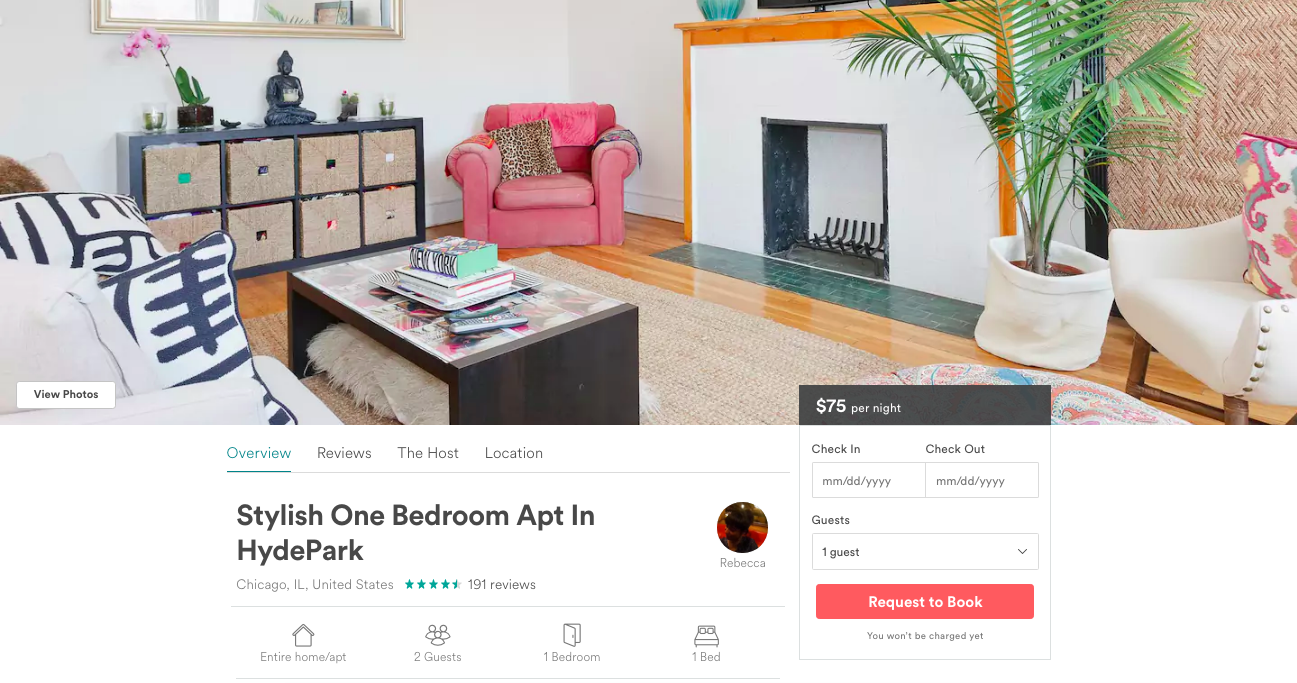
\includegraphics[width=1\textwidth]{tables/sample1-cover}
	\caption{Sample listing profile from Chicago}
\end{figure}
\begin{figure}
	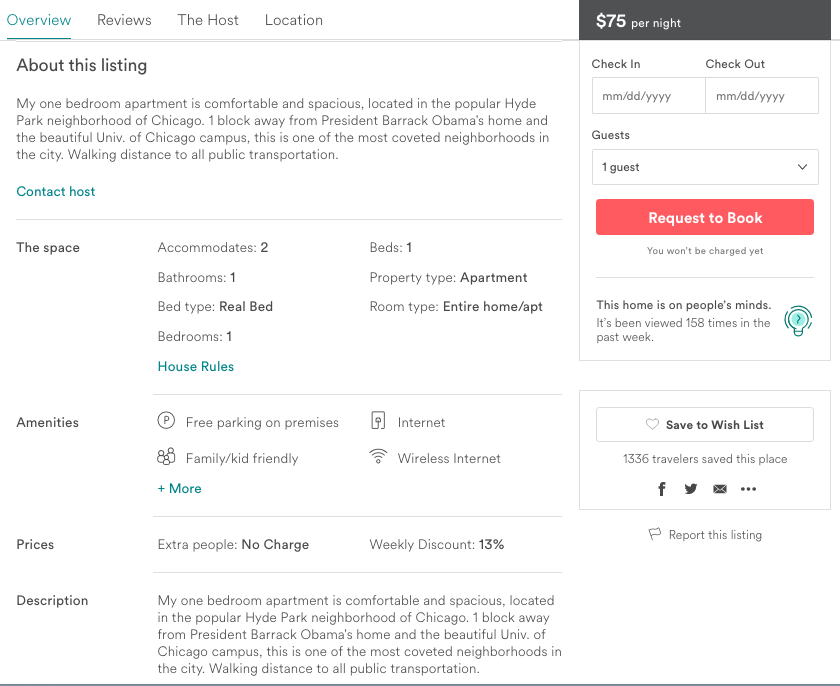
\includegraphics[width=1\textwidth]{tables/sample2-property}
	\caption{Sample property characteristics}
\end{figure}

%Histograms
\begin{figure}\centering
	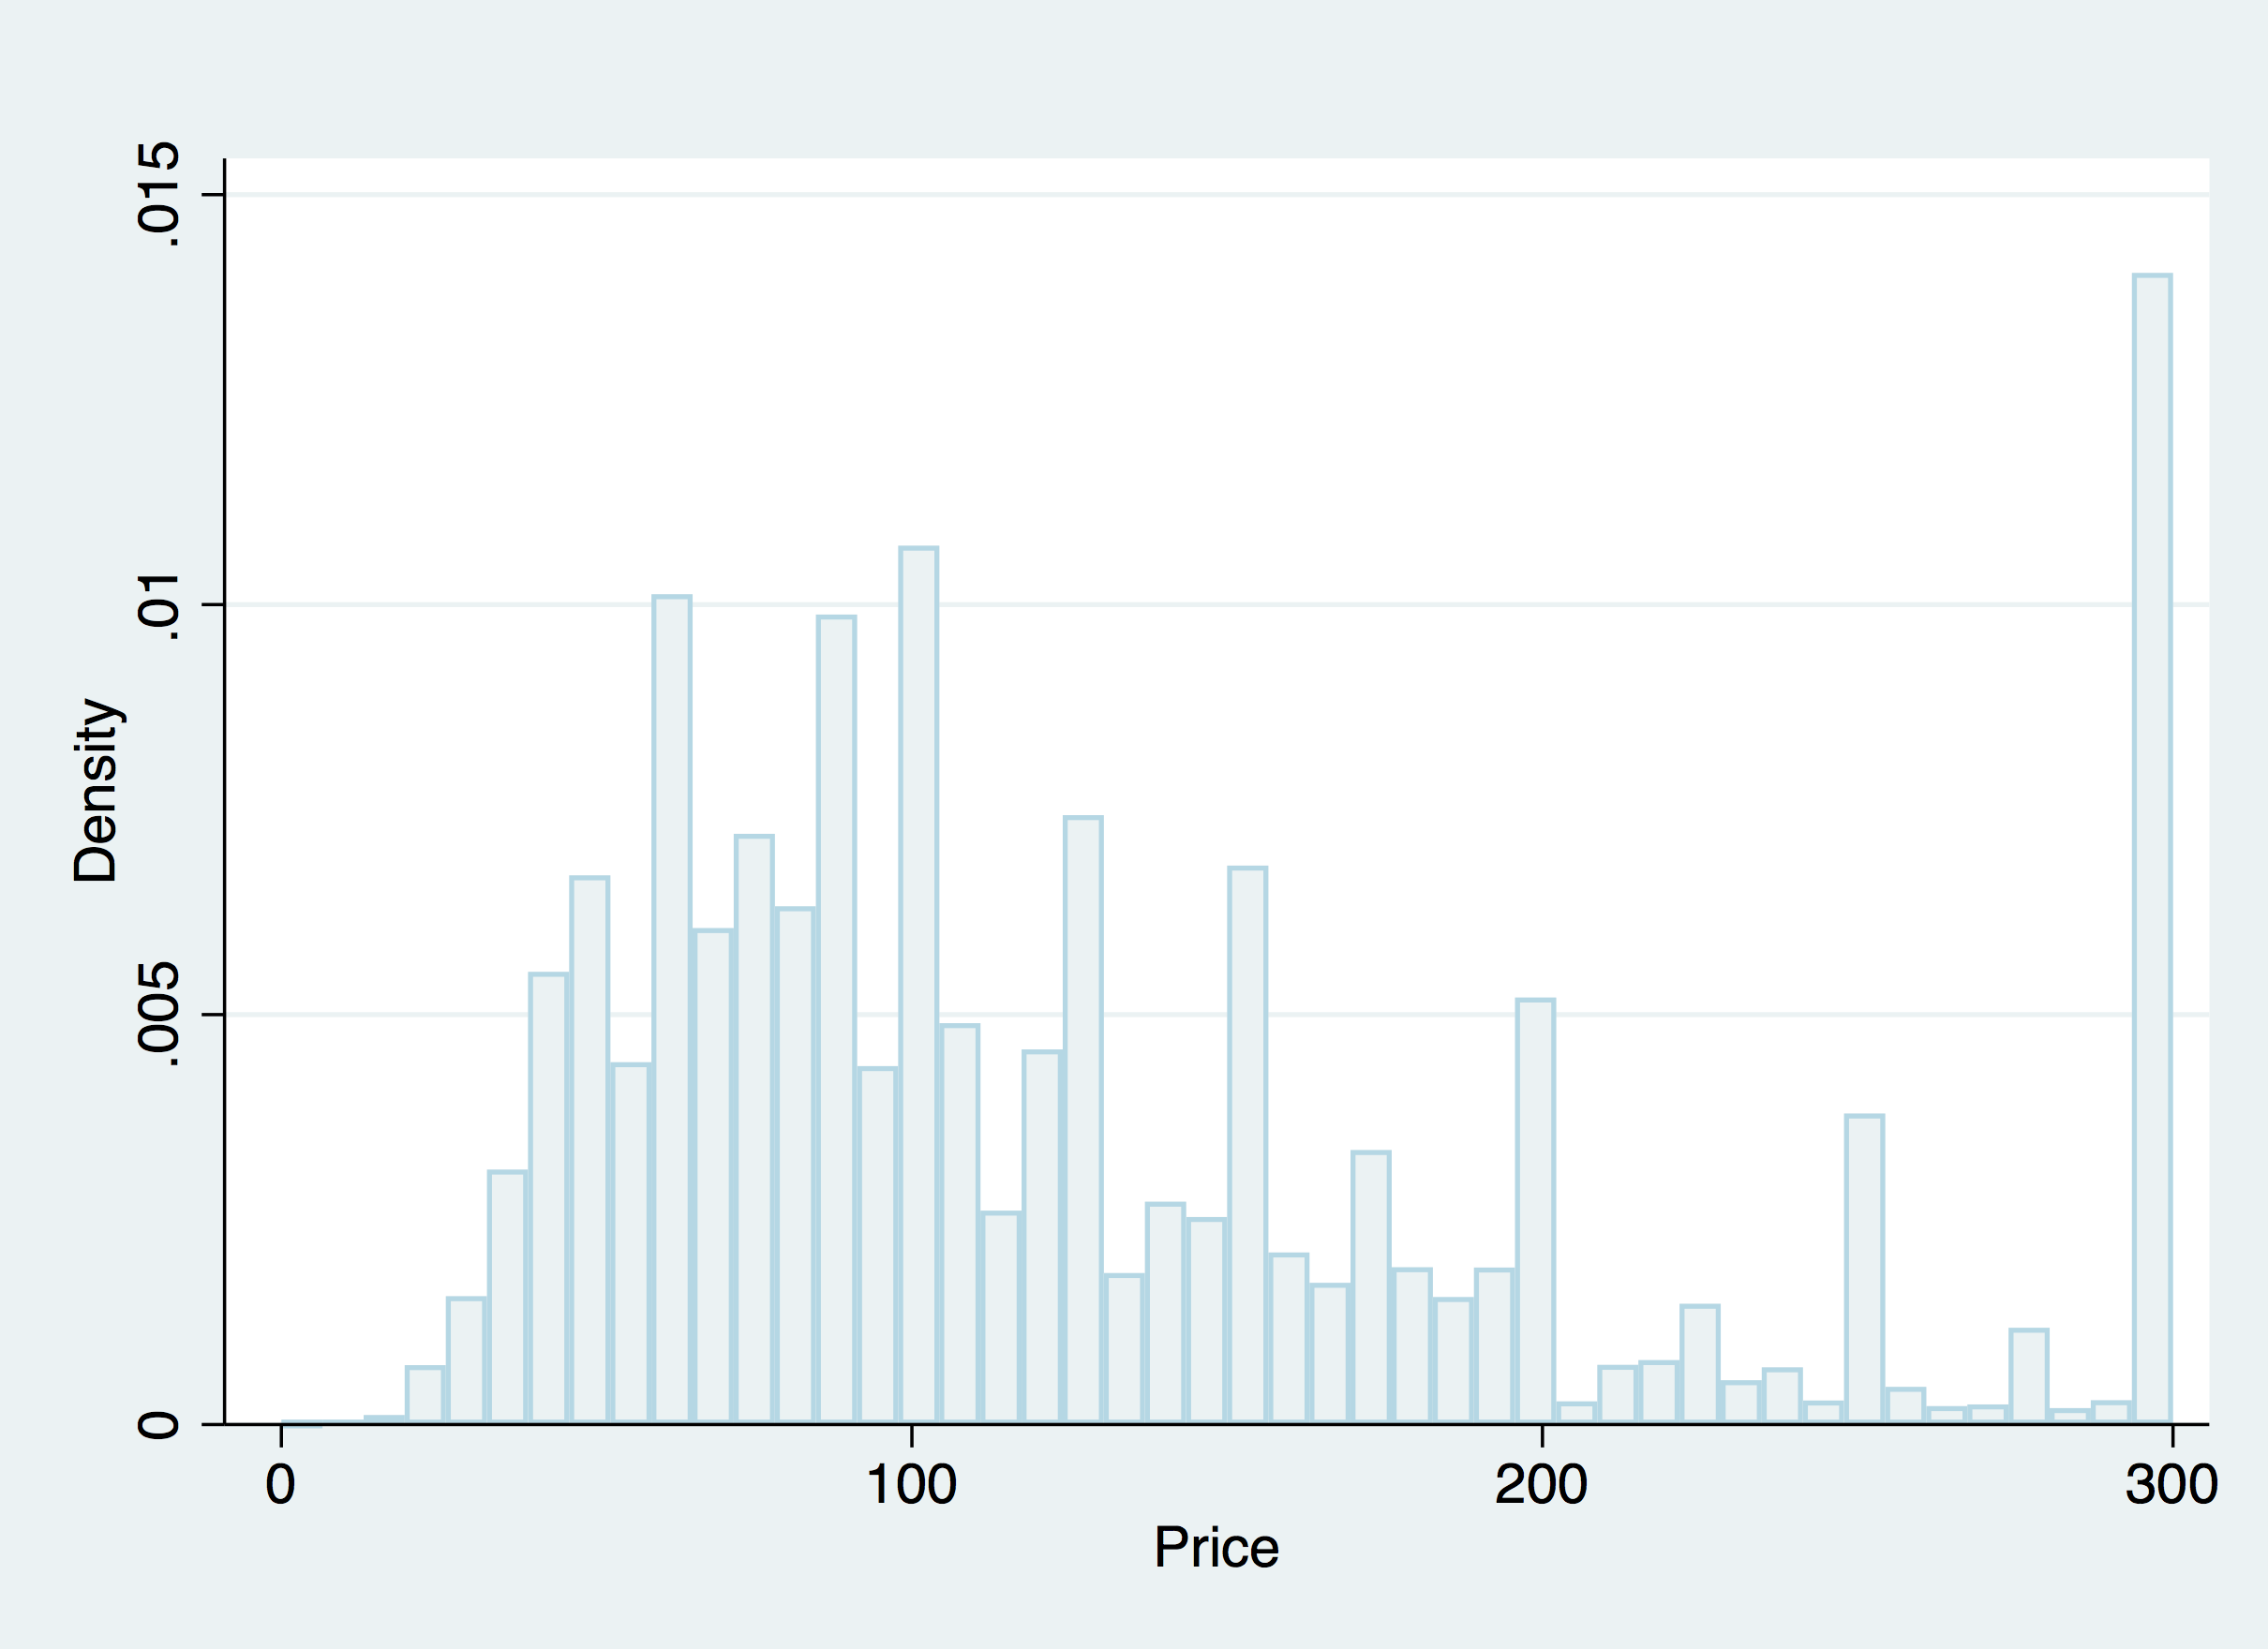
\includegraphics[width=.8\textwidth]{figures/price_dist-CONT-300}
	\caption{Distribution of prices}
	\caption*{Notes: All the listings priced at \$300 or more are grouped together at price = 300}
\end{figure}

\begin{figure}\centering
	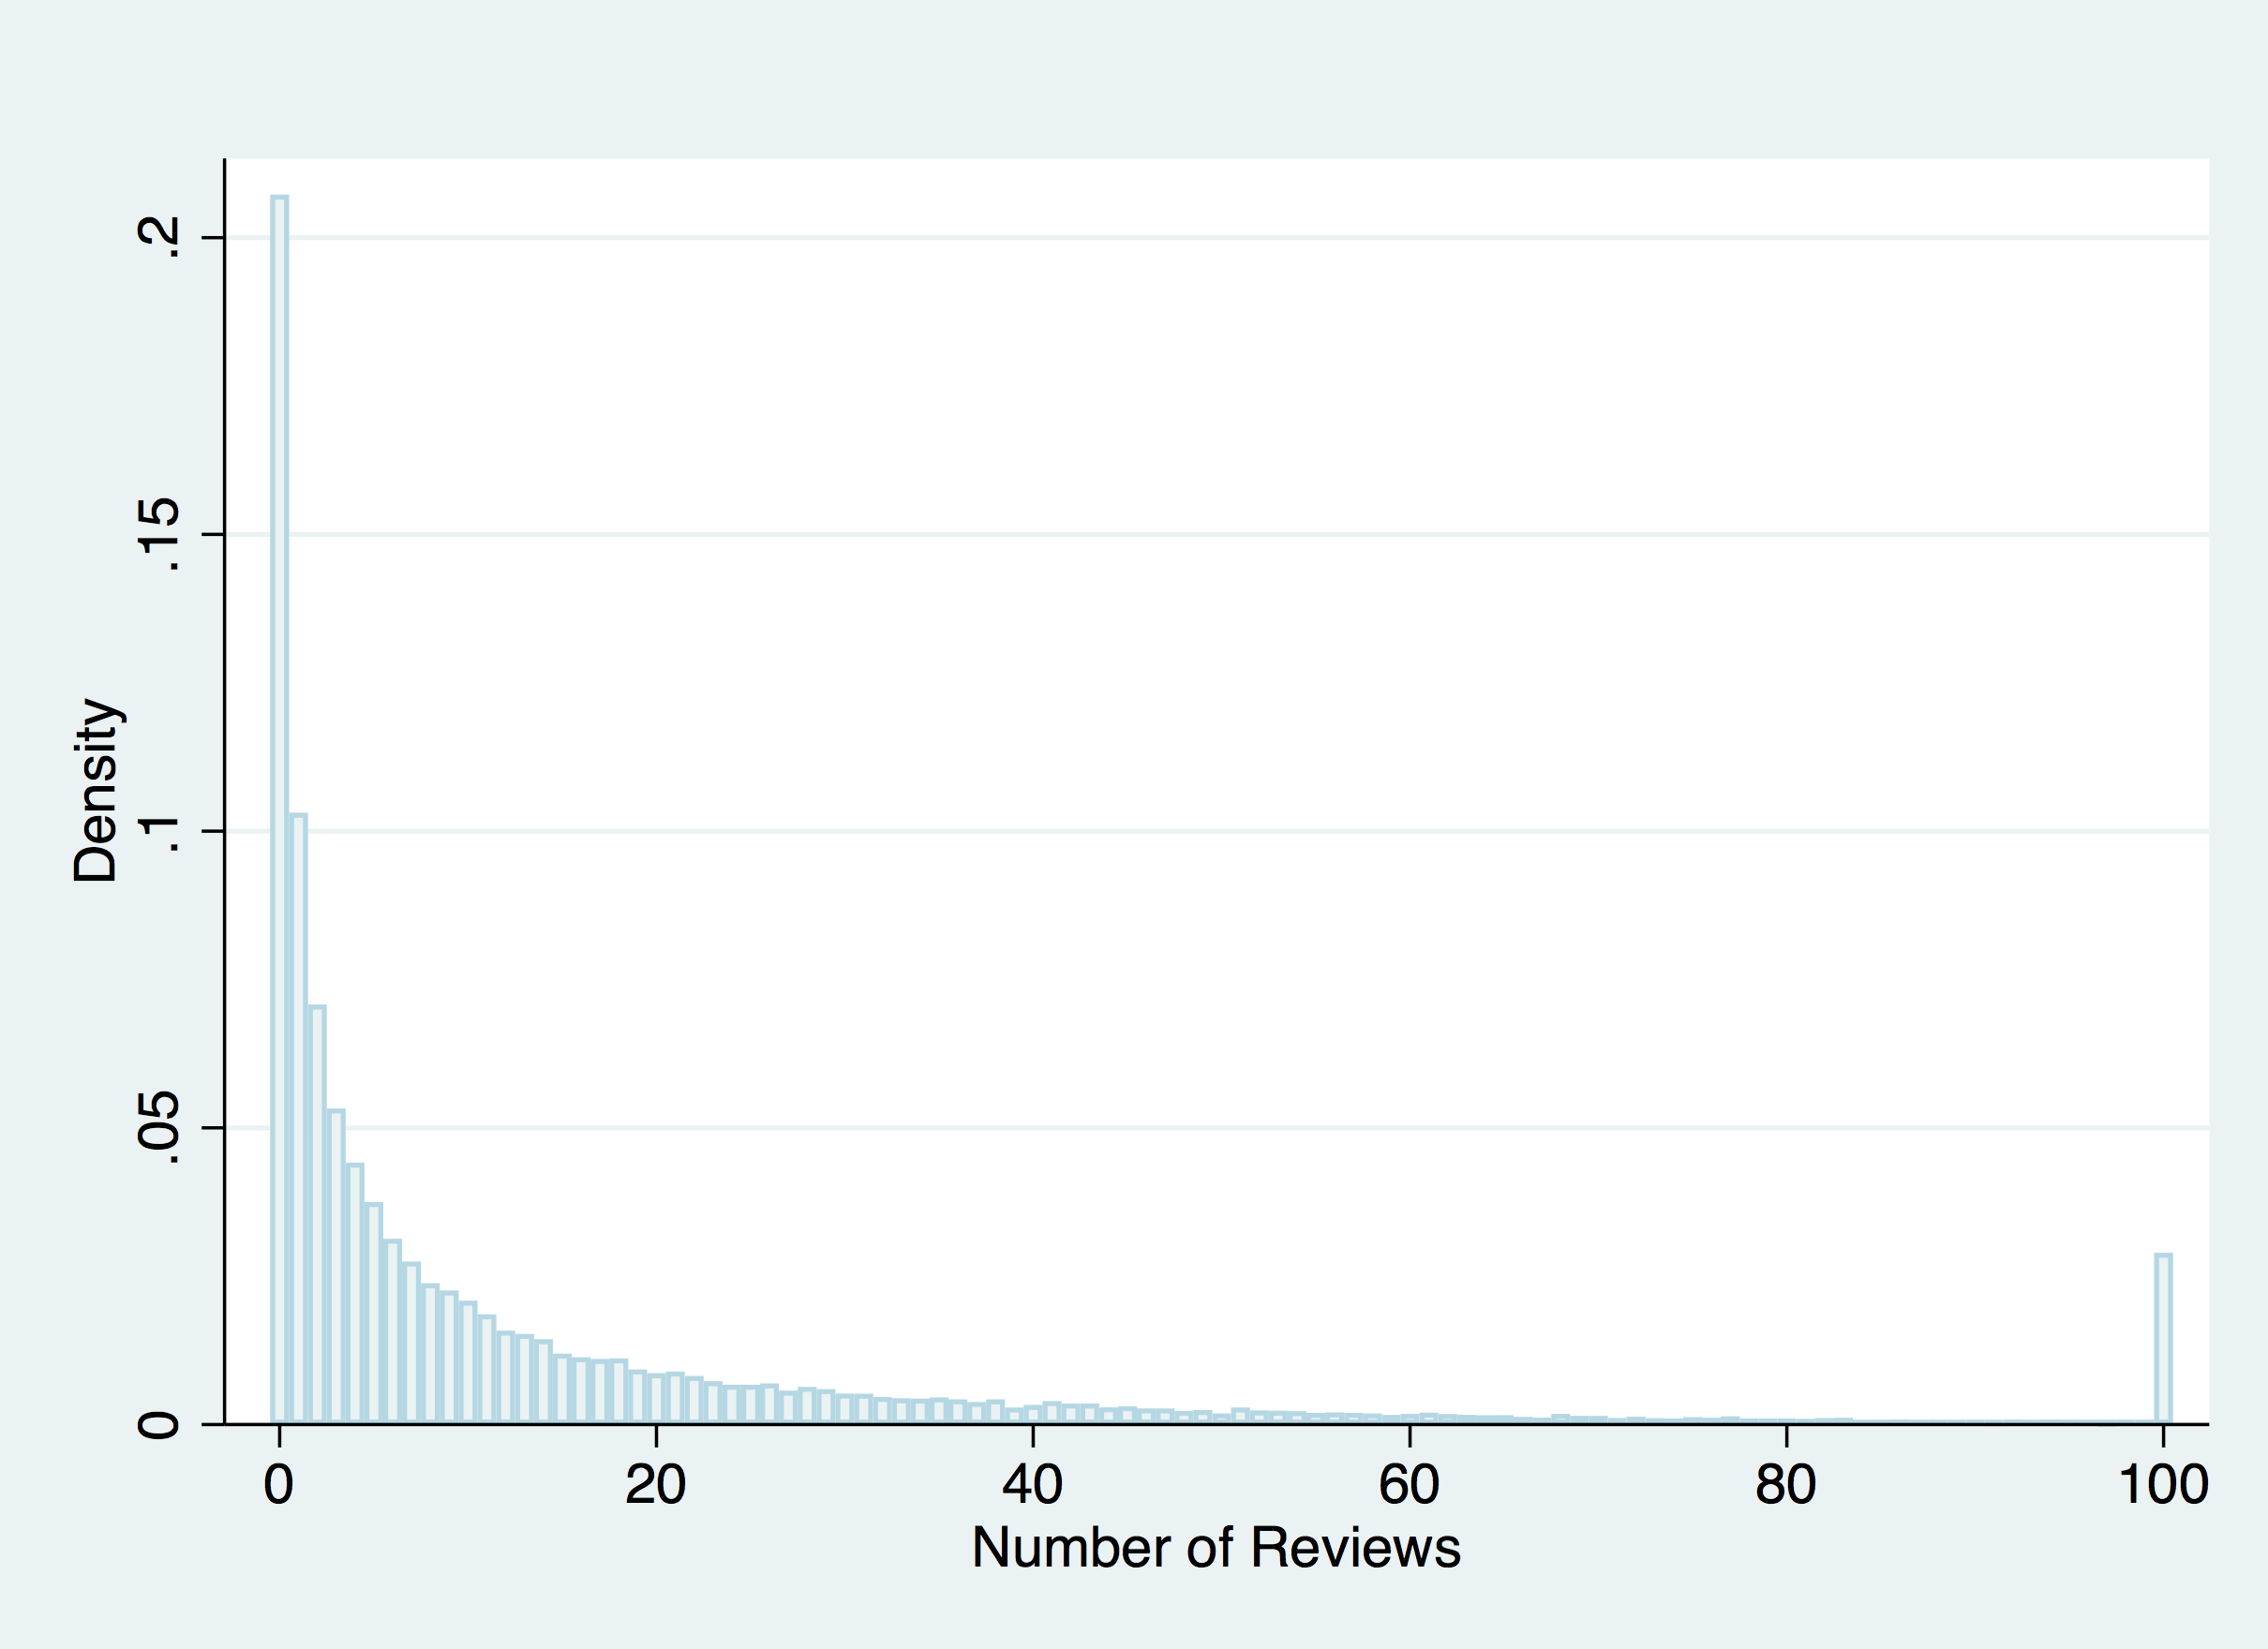
\includegraphics[width=.8\textwidth]{figures/num_reviews_dist-DISC-100}
	\caption{Distribution of number of reviews}
	\caption*{Notes: All the listings with 100 reviews or more are grouped together at number of reviews = 100}
\end{figure}

\begin{figure}\centering
	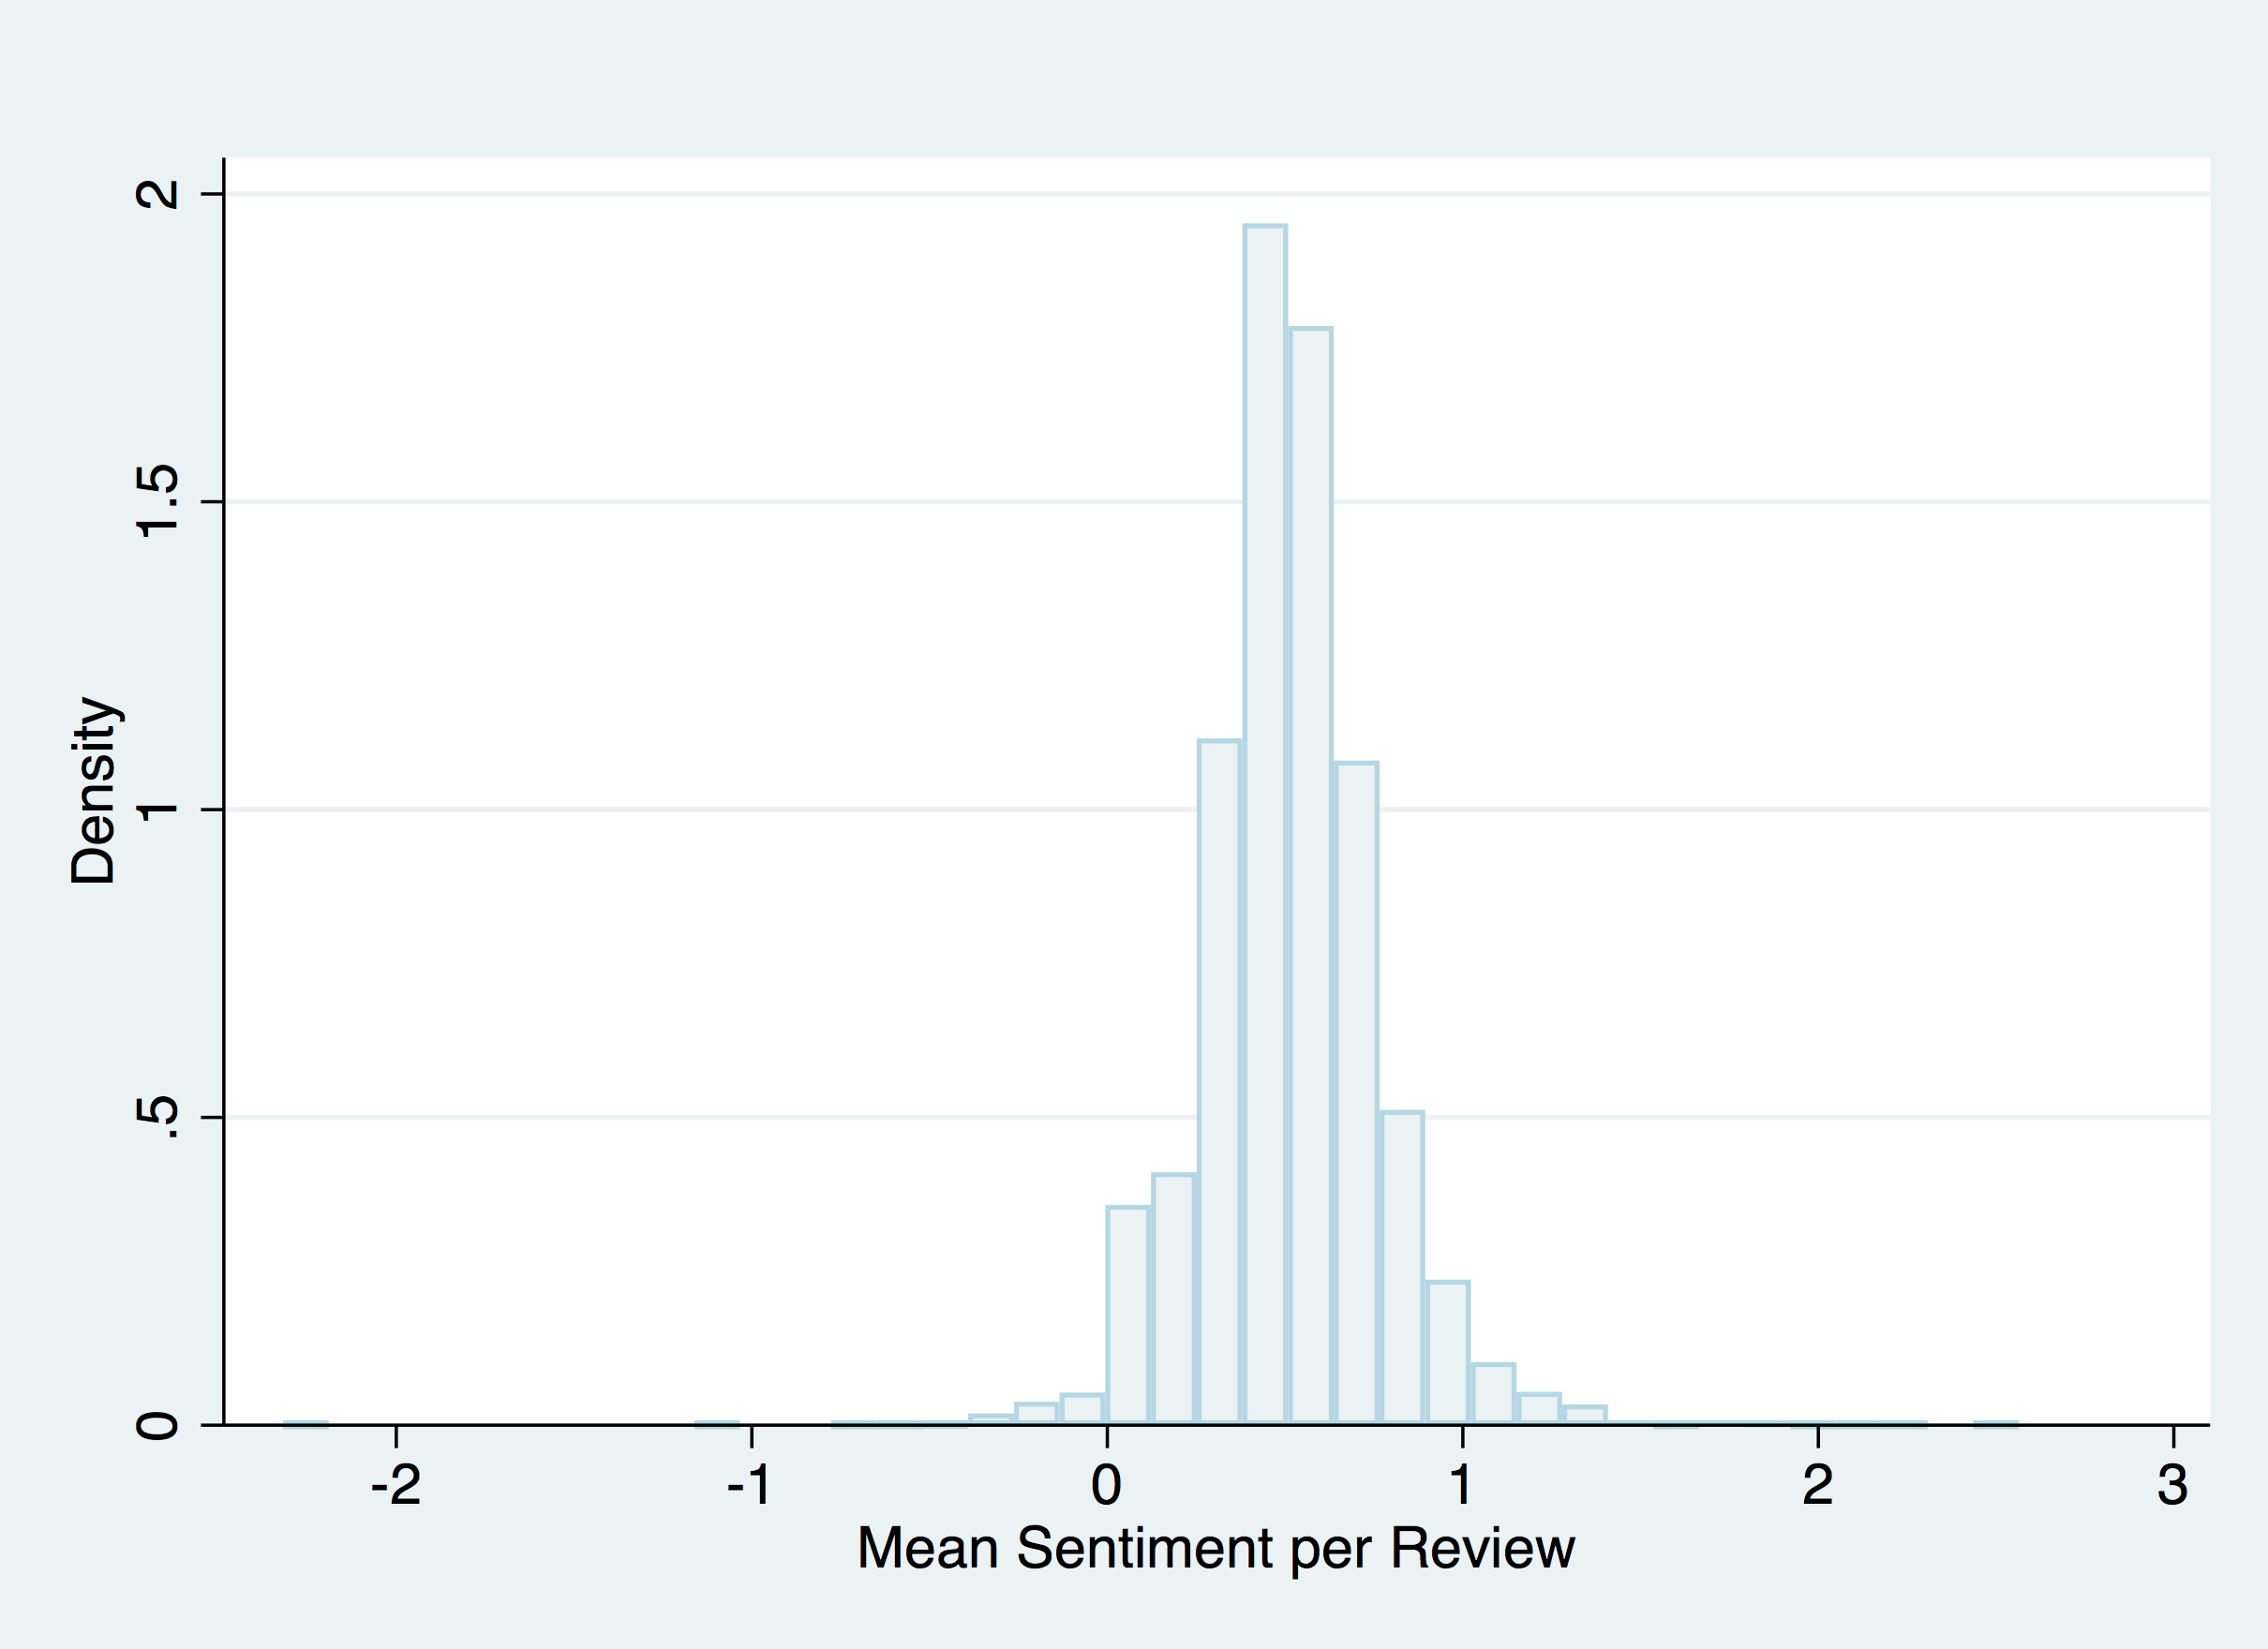
\includegraphics[width=.8\textwidth]{figures/review_sentiment_dist}
	\caption{Distribution of review sentiment}
\end{figure}


%1
%listing-level summary table
\small
{
\begin{longtable}{l*{6}{c|c|cccc}}
	\caption{Summary Statistics by Host Race: Listing Characteristics}\\
	\hline
     &\multicolumn{1}{c}{Full data}&\multicolumn{1}{c}{}&\multicolumn{1}{c}{}&\multicolumn{1}{c}{Regression sample}&\multicolumn{1}{c}{}&\multicolumn{1}{c}{}\\
      \cline{3-7}\\
     &\multicolumn{1}{c}{}&\multicolumn{1}{c}{All}&\multicolumn{1}{c}{White}&\multicolumn{1}{c}{Black}&\multicolumn{1}{c}{Hispanic}&\multicolumn{1}{c}{Asian}\\
     \hline\hline
             
\textit{Outcome variables} \\
Price (\$/day)        & 175.72  &     167.37         &      178.62      &     125.95      &     160.39       &   131.06\\
                  & (294.14) &         (277.7)         &         (289.4)         &         (208.1)         &         (275.0)     & (242.1)    \\
Number of reviews     & 17.51  &      16.57  &      17.14         &      15.06&      16.46 & 	14.08\\
                 & (31.86)  &     (30.8)         &     (31.9)         &     (27.2)         &     (29.7)        & (27.6) \\
                 
\textit{Covariates} \\
\hline
Property Type \\
\hspace{3mm} Apartments/Lofts     		&	.577 &      .598         &       .590         &      .654        &      .625 			& 	.601         \\
\hspace{3mm} Townhouses/Condos   &  .042 &      .042         &      .039         &      .041        &      .041 	& 		.055         \\
\hspace{3mm} Houses    				&.321	&      .321         &       .336        &      .279        &      .289				& 		.311         \\
\hspace{3mm} Other    				&.06	&      .039      &       .035        &      .026        &      .045	& 		.033        \\

Room Type \\
\hspace{3mm} Entire home/apt   &  .577 & .577   	&      .607	&      .449  &      .510		&    .418\\
\hspace{3mm} Private room       & .384 & 	.384		&      .363	&      .483  &      .434		&    .530\\
\hspace{3mm} Shared room      & .039 &	.04	 	&      .029	&      .067  &      .056		&    .052\\

Max Num. Guests   & 3.44   &      3.26	&      3.36  &      2.90		&    3.17 		&	 2.89\\
               & (2.41)    &     (2.3)         &     (2.3)         &     (2.1)         &     (2.4)         & (2.1)\\
Bedrooms    &  1.35 &      1.30 &      1.33         &      1.20         &      1.25   & 1.20      \\
              &   (.92)   &     (.88)         &     (.92)         &     (.72)         &     (.90)       & (.76)  \\
Bathrooms  & 1.30  &      1.27         &       1.29         &      1.20         &      1.26 & 1.21         \\
                &  (.69)  &     (.66)         &     (.68)         &     (.52)         &     (.69)         & (.58)\\
Beds       & 1.82  &      1.73 &      1.76         &      1.63         &      1.74         & 1.59\\
               &   (1.41)  &     (1.32)         &     (1.31)         &     (1.22)         &     (1.60)   & (1.21)      \\
Availability (out of 30 days)    & 11.53   &      11.30&      10.9&      14.4 &      11.46  	& 	10.88\\
         &  (10.93)    & (10.99)     &     (10.85)  &     (11.54)  &     (11.03)         &     (11.05)         \\
Number of Amenities   &   .81  &      .80		&      .81&      .77 &      .80  	& 	.75\\
         						  &  (1.10)  & (1.10)     &     (1.11)    &     (1.05)         &     (1.10)         &     (1.13)         \\
Cleaning Fee   &  67.94 &      FIX	&      .81&      .77 &      .80  	& 	.75\\
						&  (60.36)  & (FIX)     &     (1.11)         &     (1.05)         &     (1.10)     &     (1.13)         \\
Extra Guests Charge   &   13.74  &  FIX      &    .81  &      .77           &   .80  	& 	.75\\
									&  (23.65)  & (1.10)  &     (1.11) &     (1.05)     &     (1.10) &     (1.13)  \\
Instantly Bookable?   &   .15  &      FIX		&      .81&      .77 &      .80  	& 	.75\\
									&  (.361)  & (1.10)     &     (1.11)  &     (1.05)   &     (1.10)   &     (1.13)         \\
Minimum Nights   &   3.01  &      FIX		&      .81&      .77 &      .80  	& 	.75\\
							&  (9.21)  & (1.10)     &     (1.11)         &     (1.05)         &     (1.10)         &     (1.13)         \\
Strict Cancellation Policy   &   .43  &      FIX		&      .81&      .77 &      .80  	& 	.75\\
[1em]
Year of first review    & 14.86   &      FIX	&      3.36  &      2.90		&    3.17 		&	 2.89\\
							& (1.22)    &     (FIX)         &     (2.3)         &     (2.1)         &     (2.4)         & (2.1)\\

\hline
Observations  & 69,007  & 68,983   &       43,988         &       5,023         &       3,524   & 5,893      \\
\hline\hline
\caption*{Notes: The values in the table are means and standard deviations of listing-level data in my full sample. Summary statistics for selected covariates are listed in the table. Categorical variables such as room type do not have standard deviations. Property types are explicitly listed if more than 1.5\% of listings are that type. Only the most popular cancellation policy type is listed - in the full sample, 99\% of listings have strict (43\%), flexible (31\%) or moderate (25\%) cancellation policies. Year of first review is a proxy for the time on the market - 14.86 indicates that the first review of the mean listing in the full sample occured in October of 2014.}

\end{longtable}
}
\normalsize





%2
%Host-level summary table
{
	\begin{longtable}{l*{6}{c}}
		\caption{Summary Statistics by Host Race: Host Demographics}\\
		
		\hline
		&\multicolumn{1}{c}{}&\multicolumn{1}{c}{}&\multicolumn{1}{c}{}&\multicolumn{1}{c}{Regression Sample}&\multicolumn{1}{c}{}&\multicolumn{1}{c}{}\\
		\cline{3-7}\\
			&\multicolumn{1}{c}{Full data}&\multicolumn{1}{c}{All}&\multicolumn{1}{c}{White}&\multicolumn{1}{c}{Black}&\multicolumn{1}{c}{Hispanic}&\multicolumn{1}{c}{Asian}\\
		\hline\hline
		
		
		\textit{Host demographics} \\
		\hline 
		\textit{Race} \\
		\hspace{3mm}White     &.638 &      .637         &       1.00         &      0         &      0 	& 		0         \\
		\hspace{3mm}Black     & .073 &    .073       &       0         &      1.00         &      0 	& 		0         \\
		\hspace{3mm}Hispanic     &.051 &      .051         &       0         &      0         &      1.00 	& 		0         \\
		\hspace{3mm}Asian     & .085  &   .085      &       0         &      0         &      0 	& 		1.00         \\
		\hspace{3mm}Unknown     &.153 &      .152         &       0         &      0         &      0 	& 		0         \\
		[1em]
		\textit{Sex} \\
		\hspace{3mm}Male     & .310 &      .309         &       .356         &      .354         &      .417 	& 		.367        \\
		\hspace{3mm}Female     &.378 &      .378         &       .427        &      .541         &      .426 	& 		.476         \\
		\hspace{3mm}Unknown   & .312 &      .312         &       .216         &      .104         &      .156 	& 		.157         \\
		[1em]
		\textit{Age} \\
		\hspace{3mm}Young ($<$ 30)     &.427 &      .427         &       .469         &      .514        &      .481 	& 		.587         \\
		\hspace{3mm}Middle-aged     & .421&      .421         &       .491        &      .470         &      .490 		& 		.379         \\
		\hspace{3mm}Old ($>$ 65)     & .019&      .018         &       .026         &      .004         &      .009	& 		.009         \\
		\hspace{3mm}Unknown    &  .133&      .133    &       .013         &      .011         &      .018 	& 		.024         \\
		[1em]

		
		\hline
		Observations    &69,007  & 68,983   &       43,988         &       5,023         &       3,524         &       5,893         \\
		\hline\hline
		\caption*{Notes: The values in the table are means and standard deviations of host-level data in my full sample. Summary statistics for selected covariates are listed in the table. Categorical variables such as race, sex, and age do not have standard deviations. White refers only to Non-Hispanic Whites.}
		
	\end{longtable}
}



%3
%Host-level summary table
{
	\begin{longtable}{l*{6}{c}}
		\caption{Summary Statistics by Host Race: Host Characteristics}\\
		
		\hline
		&\multicolumn{1}{c}{}&\multicolumn{1}{c}{}&\multicolumn{1}{c}{}&\multicolumn{1}{c}{Regression Sample}&\multicolumn{1}{c}{}&\multicolumn{1}{c}{}\\
		\cline{3-7}\\
			&\multicolumn{1}{c}{Full data}&\multicolumn{1}{c}{All}&\multicolumn{1}{c}{White}&\multicolumn{1}{c}{Black}&\multicolumn{1}{c}{Hispanic}&\multicolumn{1}{c}{Asian}\\
		\hline\hline           
		     
		\textit{Outcome variables} \\
		
		Host listings count         & 6.38 &      5.53&      5.50 &      10.5&    3.16 & 2.68\\
		& (36.54)	&     (33.0)         &     (31.2)         &     (60.3)         &     (17.8) & 	(3.62)         \\
		
		\textit{Covariates} \\

		\hline
		Review value out of 100      & 93.56  &      93.61	&      94.08	 	&      91.89		&    92.81	 & 		92.24\\
		              &   (8.13)   &     (8.00)         &     (7.49)         &     (9.42)         &     (8.72) 	&	 (9.27)         \\
		
		Host is a superhost    & .135   &      .124		&      .134&      .084 &      .108  	& 	.097\\
		&(.341) & (.329)     &     (.341)         &     (.277)         &     (.310)         &     (.296)         \\

		Response rate      & .933  &       .756		&       .756		&      .771         &      .756  	& 	.744\\
		& (.160) &     (.391)         &     (.393)         &     (.368)         &     (.386)         &		(.399)\\

		Response time $<$ 1 hour      & .411  &       .756		&       .756		&      .771         &      .756  	& 	.744\\

		Acceptance rate      & .882    &      .453&      .463&       .357         &      .494    &	.446     \\
		&.204 &     (.463)         &     (.463)         &     (.451)         &     (.466)         &		(.467)\\

		Total ``good" words       & .640   &      .655&      .656&       .686         &      .677    &	.604     \\
		& (.839) &     (.857)         &     (.843)         &     (.882)         &     (.867)         &		(.826)\\

		Length of ``Summary"      &   208.661  &      208.67 	&      210.20	&       203.25         &      206.74    &	205.81     \\
		&(65.00) &       (64.99)  &    (64.08)         &     (70.59)         &     (65.62)         &     (65.87) \\

		Short words in ``Summary"          & .158 &      .182		&      .185		&       .187         &      .175    &	.175     \\
		&(.041) &     (1.19)         &     (1.15)         &     (1.24)         &     (1.26)         &		(1.32)\\                    

		Host's Identity Verified?          & .705 &      FIX		&      .185		&       .187         &      .175    &	.175     \\
		&(.456) &     (FIX)         &     (1.15)         &     (1.24)         &     (1.26)         &		(1.32)\\                    

		Guest Pic Required?   &   .039  &      .80		&      .81&      .77 &      .80  	& 	.75\\
		&  (.194)  & (1.10)     &     (1.11)         &     (1.05)         &     (1.10)         &     (1.13)         \\
		Guest Phone Required?   &   .050  &      .80		&      .81&      .77 &      .80  	& 	.75\\
		&  (.218)  & (1.10)     &     (1.11)         &     (1.05)         &     (1.10)         &     (1.13)         \\
		
		
		\hline
		Observations (full sample)    & 69,007  & 68,983   &       43,988         &       5,023         &       3,524         &       5,893         \\
		\hline\hline
		\caption*{Notes: The values in the table are means and standard deviations of host-level data in my full sample. Summary statistics for selected covariates are listed in the table. Categorical variables such as race, sex, and age do not have standard deviations. White refers only to Non-Hispanic Whites. Length of ``Summary" and proportion of short words in the ``Summary'' refer to my constructed measures of host quality. These two measures were also calculated for the description, space, neighborhood overview, notes, and transit fields, but were not included in the table for the sake of clarity and because they follow a similar pattern as the ``Summary" field. Statistics for only the most frequent response time (``within an hour") were included.}
		
	\end{longtable}
}


%4
% reviewer summary table

{
	\begin{longtable}{l*{5}{c}}
		\caption{Summary Statistics by Race: Reviewer Characteristics}\\
		\hline
		&\multicolumn{1}{c}{(1)}&\multicolumn{1}{c}{(2)}&\multicolumn{1}{c}{(3)}&\multicolumn{1}{c}{(4)}&\multicolumn{1}{c}{(5)}\\
		&\multicolumn{1}{c}{Full sample}&\multicolumn{1}{c}{White}&\multicolumn{1}{c}{Black}&\multicolumn{1}{c}{Hispanic}&\multicolumn{1}{c}{Asian}\\
		\hline\hline                

		\textit{Reviewer characteristics} \\
		\hline
		Host race            &      1.00 &      .738&       .099         &      .079    &	.083     \\
		[1em]
		Reviewer race            &      1.00		&      .759	&       .041         &      .047    &	.153     \\
		[1em]
		Review sentiment            &      .510	&      .512&       .503         &      .509    &	.506     \\
		&     (.261)         &     (.254)         &     (.258)         &     (.276)         &		(.287)\\
		[1em]
		Listing sentiment            &      .507&      .509&       .502         &      .499    &	.506     \\
		&     (.072)         &     (.067)         &     (.089)         &     (.096)         &		(.094)\\
		
		\hline
		Observations (full sample)     & FIX 68,983   &       43,988         &       5,023         &       3,524         &       5,893         \\
		\hline\hline
		\caption*{Notes: The values in the table are means and standard deviations of reviewer-level data of a randomly chosen set of hosts in Chicago. Categorical variables do not have standard deviations. White refers only to Non-Hispanic Whites. The host race and the reviewer race is the proportion of each race included in the reviewer sample. The review sentiment is the sentiment of each review, the listing sentiment is the average sentiment per listing.}
		
	\end{longtable}
}



%5 - Main
{
\def\sym#1{\ifmmode^{#1}\else\(^{#1}\)\fi}
\begin{longtable}{l*{4}{c}}
\caption{Main result: Estimates of effect of host's race and gender on price}\\
\hline\hline\endfirsthead\hline\endhead\hline\endfoot\endlastfoot
                    &\multicolumn{1}{c}{(1)}&\multicolumn{1}{c}{(2)}&\multicolumn{1}{c}{(3)}&\multicolumn{1}{c}{(4)}\\
                    &\multicolumn{1}{c}{Price}&\multicolumn{1}{c}{Price}&\multicolumn{1}{c}{Price}&\multicolumn{1}{c}{Price}\\
\hline
White Female        &      -3.727\sym{*}  &      -3.714\sym{*}  &      -0.827         &      -0.243         \\
                    &     (1.770)         &     (1.562)         &     (1.049)         &     (1.053)         \\
[1em]
Black Male          &      -39.43\sym{***}&      -14.24\sym{***}&      -6.891\sym{***}&      -6.917\sym{***}\\
                    &     (4.058)         &     (3.483)         &     (1.994)         &     (1.963)         \\
[1em]
Black Female        &      -41.69\sym{***}&      -11.20\sym{***}&      -6.271\sym{***}&      -5.793\sym{***}\\
                    &     (4.315)         &     (2.793)         &     (1.577)         &     (1.586)         \\
[1em]
Hispanic Male       &      -20.59\sym{***}&      -7.247\sym{**} &      -2.537         &      -2.165         \\
                    &     (3.727)         &     (2.759)         &     (2.051)         &     (2.073)         \\
[1em]
Hispanic Female     &      -23.05\sym{***}&      -11.38\sym{***}&      -5.284\sym{*}  &      -5.022\sym{*}  \\
                    &     (4.426)         &     (3.219)         &     (2.110)         &     (2.078)         \\
[1em]
Asian Male          &      -27.42\sym{***}&      -12.08\sym{***}&      -5.834\sym{**} &      -6.338\sym{**} \\
                    &     (4.954)         &     (3.553)         &     (2.206)         &     (2.185)         \\
[1em]
Asian Female        &      -39.18\sym{***}&      -21.20\sym{***}&      -8.611\sym{***}&      -8.604\sym{***}\\
                    &     (4.463)         &     (2.592)         &     (1.586)         &     (1.599)         \\
[1em]
Constant            &       147.4\sym{***}&       54.75\sym{***}&      -33.93\sym{***}&      -0.742         \\
                    &     (5.015)         &     (1.506)         &     (5.507)         &     (6.764)         \\
\hline
Controls:        \\
\hspace{3mm} Location  &                &       X         &       X         &       X         \\
\hspace{3mm} Property Characteristics  &                &                &       X         &       X         \\
\hspace{3mm} Host Characteristics  &                &                &                &       X         \\
\hline
Observations        &       45072         &       45072         &       45072         &       45072         \\
Adjusted \(R^{2}\)  &       0.019         &       0.166         &       0.621         &       0.627         \\
\hline\hline
\multicolumn{5}{l}{\footnotesize Standard errors in parentheses}\\
\multicolumn{5}{l}{\footnotesize \sym{*} \(p<0.05\), \sym{**} \(p<0.01\), \sym{***} \(p<0.001\)}\\
\caption*{Notes: The dependent variable is the price of the listing. All race coefficients are relative to white males. The unit of observation is a listing. The sample is the sample of listings across 7 US cities. Model 1 is the baseline effect of host demographics on price. Model 2 controls for listing location to the neighborhood level. Model 3 adds listing characteristics such as property type, time on market, number of bedrooms, availability, etc. Model 4 adds host characteristics such as response and acceptance rates, measures of host effort, Superhost status, etc. See Data Appendix for full description of covariates.}
\label{Table 4}


\end{longtable}
}


\begin{comment}
[1em]
Middle-aged         &       12.21\sym{***}&       10.62\sym{***}&       1.724         &       1.702         \\
&     (2.126)         &     (1.281)         &     (0.913)         &     (0.907)         \\
[1em]
Old ($>$ 65)           &       8.145         &       3.664         &      -1.752         &      -2.239         \\
&     (5.936)         &     (5.339)         &     (3.271)         &     (3.237)         \\
	
\end{comment}


%6
{
\def\sym#1{\ifmmode^{#1}\else\(^{#1}\)\fi}
\begin{longtable}{l*{1}{c}}
\caption{Robustness check with controls from Edelman \& Luca (2014), NYC data}\\
\hline\hline\endfirsthead\hline\endhead\hline\endfoot\endlastfoot
                    &\multicolumn{1}{c}{(1)}\\
                    &\multicolumn{1}{c}{Price per night}\\
\hline
Black               &      -18.11\sym{***}\\
                    &     (1.813)         \\
Accommodates        &       12.84\sym{***}\\
                    &     (0.488)         \\
Bedrooms            &       33.60\sym{***}\\
                    &     (1.227)         \\
Review Scores Location&      -74.66\sym{***}\\
                    &     (7.363)         \\
Review Scores Location Squared           &       5.407\sym{***}\\
                    &     (0.421)         \\

Review Scores Checkin&      -1.268         \\
                    &     (1.157)         \\
Review Scores Communication&      -1.226         \\
                    &     (1.218)         \\
Review Scores Cleanliness&       3.454\sym{***}\\
                    &     (0.706)         \\
Review Scores Accuracy&      -1.479         \\
                    &     (0.973)         \\
Host verified &       1.945         \\
                    &     (1.357)         \\
Private room        &      -71.14\sym{***}\\
                    &     (1.400)         \\
Shared room         &      -102.8\sym{***}\\
                    &     (3.109)         \\
\hline
Controls:        \\
\hspace{3mm} Location  &                           X      \\
\hspace{3mm} Property Characteristics  &   X         \\
\hspace{3mm} Host Characteristics  &         X        \\
\hline
Observations        &       11999         \\
Adjusted \(R^{2}\)  &       0.526         \\
\hline\hline
\multicolumn{2}{l}{\footnotesize Standard errors in parentheses}\\
\multicolumn{2}{l}{\footnotesize \sym{*} \(p<0.05\), \sym{**} \(p<0.01\), \sym{***} \(p<0.001\)}\\
\caption*{Notes: This table presents the effect on price of controlling for Edelman \& Luca's (2014) full specification using my NYC data. The results are nearly identical to theirs (their coefficient on black hosts was -17.8) when controlling for similar covariates in the same city. The omitted category for race is white hosts. The omitted category for room type is Entire Apartment. I could not control for host social media accounts as a proxy for host reliability like Edelman \& Luca, because Airbnb no longer provides this information. Instead, I controlled for ``host verified", a boolean for whether Airbnb has the host's phone number and email. I was not able to control for ``picture quality", but picture quality did not significantly influence price in Edelman \& Luca's regression.}\\
\end{longtable}
}




%7
{
\def\sym#1{\ifmmode^{#1}\else\(^{#1}\)\fi}
\begin{longtable}{l*{4}{c}}
\caption{Estimates of effect of host's race and gender on number of reviews}\\
\hline\hline\endfirsthead\hline\endhead\hline\endfoot\endlastfoot
                    &\multicolumn{1}{c}{(1)}&\multicolumn{1}{c}{(2)}&\multicolumn{1}{c}{(3)}&\multicolumn{1}{c}{(4)}\\
                    &\multicolumn{1}{c}{Num Reviews}&\multicolumn{1}{c}{Num Reviews}&\multicolumn{1}{c}{Num Reviews}&\multicolumn{1}{c}{Num Reviews}\\
\hline
White Female        &      -0.804         &      -0.560         &      -1.420\sym{***}&      -1.362\sym{***}\\
                    &     (0.540)         &     (0.496)         &     (0.344)         &     (0.338)         \\
[1em]
Black Male          &      -2.049         &      -1.494         &      -2.034\sym{**} &      -1.287\sym{*}  \\
                    &     (1.137)         &     (0.970)         &     (0.617)         &     (0.599)         \\
[1em]
Black Female        &      -2.153         &      -1.439         &      -2.523\sym{***}&      -2.330\sym{***}\\
                    &     (1.125)         &     (1.004)         &     (0.559)         &     (0.536)         \\
[1em]
Hispanic Male       &      -1.404         &      -0.168         &      -0.183         &    -0.00232         \\
                    &     (1.258)         &     (1.178)         &     (0.817)         &     (0.797)         \\
[1em]
Hispanic Female     &      -0.443         &       0.805         &      -0.867         &      -0.462         \\
                    &     (1.119)         &     (1.042)         &     (0.749)         &     (0.704)         \\
[1em]
Asian Male          &      -2.856\sym{**} &      -1.054         &      -1.024         &      -1.030         \\
                    &     (0.913)         &     (0.832)         &     (0.606)         &     (0.557)         \\
[1em]
Asian Female        &      -3.112\sym{**} &      -0.818         &      -1.201\sym{*}  &      -0.940         \\
                    &     (0.952)         &     (0.770)         &     (0.598)         &     (0.565)         \\
[1em]
Constant            &       15.49\sym{***}&       27.80\sym{***}&       130.1\sym{***}&       114.8\sym{***}\\
                    &     (0.559)         &     (0.474)         &     (2.409)         &     (2.853)         \\
\hline
Controls:        \\
\hspace{3mm} Location  &                &       X         &       X         &       X         \\
\hspace{3mm} Property Characteristics  &                &                &       X         &       X         \\
\hspace{3mm} Host Characteristics  &                &                &                &       X         \\
\hline
Observations        &       45072         &       45072         &       45072         &       45072         \\
Adjusted \(R^{2}\)  &       0.009         &       0.049         &       0.398         &       0.443         \\
\hline\hline
\multicolumn{5}{l}{\footnotesize Standard errors in parentheses}\\
\multicolumn{5}{l}{\footnotesize \sym{*} \(p<0.05\), \sym{**} \(p<0.01\), \sym{***} \(p<0.001\)}\\
\caption*{Notes: The dependent variable is the number of reviews of the listing. The omitted category for race is white males, so all coefficients are relative to that group. The unit of observation is an Airbnb listing, so hosts who have multiple listings are treated separately each time. The sample is the sample of listings across 7 US cities. The specification is the same as Table 5. See Data Appendix for a discussion of my covariates.}
\end{longtable}
}


\begin{comment}
[1em]
Middle-aged         &       4.358\sym{***}&       5.298\sym{***}&       0.634         &      -0.101         \\
&     (0.585)         &     (0.562)         &     (0.371)         &     (0.361)         \\
[1em]
Old ($>$65)           &       13.30\sym{***}&       14.75\sym{***}&       2.328         &       0.741         \\
&     (2.130)         &     (1.981)         &     (1.358)         &     (1.265)         \\
\end{comment}


%8
{
\def\sym#1{\ifmmode^{#1}\else\(^{#1}\)\fi}
\begin{longtable}{l*{1}{c}}
\caption{Effect of host's race on listing availability out of 30 days}\\
\hline\hline\endfirsthead\hline\endhead\hline\endfoot\endlastfoot
                    &\multicolumn{1}{c}{(1)}\\
                    &\multicolumn{1}{c}{Number of vacant days out of 30}\\
\hline
White Female        &      -0.861\sym{***}\\
                    &     (0.114)         \\
[1em]
Black Male          &       2.317\sym{***}\\
                    &     (0.308)         \\
[1em]
Black Female        &       1.785\sym{***}\\
                    &     (0.277)         \\
[1em]
Hispanic Male       &      -0.154         \\
                    &     (0.331)         \\
[1em]
Hispanic Female     &     -0.0906         \\
                    &     (0.341)         \\
[1em]
Asian Male          &      -0.195         \\
                    &     (0.299)         \\
[1em]
Asian Female        &      -1.191\sym{***}\\
                    &     (0.259)         \\
\hline
Controls:        \\
\hspace{3mm} Location  &                           X      \\
\hspace{3mm} Property Characteristics  &   X         \\
\hspace{3mm} Host Characteristics  &         X        \\
\hline
Observations        &       45779         \\
Adjusted \(R^{2}\)  &       0.215         \\
\hline\hline
\multicolumn{2}{l}{\footnotesize Standard errors in parentheses}\\
\multicolumn{2}{l}{\footnotesize \sym{*} \(p<0.05\), \sym{**} \(p<0.01\), \sym{***} \(p<0.001\)}\\
\caption*{Notes: This table presents the effect of host race on listing availability out of 30 days, controlling for my preferred specification throughout. When a listing is booked, this availability metric is updated on the Airbnb website to reflect that booking. Therefore, this measure actually represents the number of days out of the total available days that listings were vacant, relative to white male hosts.}\\
\end{longtable}
}




%9
{
\def\sym#1{\ifmmode^{#1}\else\(^{#1}\)\fi}
\begin{longtable}{l*{7}{c}}
\caption{Robustness checks by city}\\
\hline\hline\endfirsthead\hline\endhead\hline\endfoot\endlastfoot
                    &\multicolumn{1}{c}{(1)}&\multicolumn{1}{c}{(2)}&\multicolumn{1}{c}{(3)}&\multicolumn{1}{c}{(4)}&\multicolumn{1}{c}{(5)}&\multicolumn{1}{c}{(6)}&\multicolumn{1}{c}{(7)}\\
                    &\multicolumn{1}{c}{LA}&\multicolumn{1}{c}{NYC}&\multicolumn{1}{c}{Austin}&\multicolumn{1}{c}{Chicago}&\multicolumn{1}{c}{New Orleans}&\multicolumn{1}{c}{DC}&\multicolumn{1}{c}{Nashville}\\
\hline
Black               &      -5.156\sym{*}  &      -3.977\sym{*}  &      -6.284         &      -2.942         &      -18.45\sym{*}  &      -7.426         &      -4.754         \\
                    &     (2.144)         &     (1.692)         &     (10.75)         &     (3.181)         &     (8.203)         &     (4.872)         &     (8.193)         \\
[1em]
Hispanic            &      -5.621\sym{*}  &      -1.246         &       0.877         &      -0.807         &       4.109         &       3.264         &      -38.58\sym{***}\\
                    &     (2.197)         &     (1.937)         &     (5.212)         &     (5.180)         &     (10.77)         &     (4.739)         &     (9.458)         \\
[1em]
Asian               &      -5.585\sym{**} &      -5.975\sym{**} &      -27.66\sym{***}&      -17.64\sym{***}&       3.805         &      -5.880         &       10.50         \\
                    &     (1.785)         &     (2.043)         &     (7.763)         &     (4.353)         &     (13.36)         &     (3.131)         &     (21.29)         \\
\hline
Observations        &       16825         &       14765         &        3636         &        3255         &        2563         &        2285         &        1747         \\
Adjusted \(R^{2}\)  &       0.684         &       0.616         &       0.611         &       0.613         &       0.568         &       0.586         &       0.670         \\
\hline\hline
\multicolumn{8}{l}{\footnotesize Standard errors in parentheses}\\
\multicolumn{8}{l}{\footnotesize \sym{*} \(p<0.05\), \sym{**} \(p<0.01\), \sym{***} \(p<0.001\)}\\
\caption*{Notes: The dependent variable is the price of a listing. This table breaks down the combined effects shown in the last column of Table 3 by city. The omitted category for race is White hosts, so all coefficients are relative to that group. For ease of reading, I did not include the gender of the host. I control for my preferred specification (referred to as Model 4 in Table 3) that includes host demographics, listing location, listing characteristics, and host characteristics. See Section 3.1 for a full discussion of the covariates included. Low number of observations for Black, Hispanic, and Asian hosts contribute to imprecise estimates in cities with less than 5,000 Airbnb hosts (New Orleans and Nashville have less than 100 Hispanic and Asian hosts, DC and Austin have less than 200 Hispanic and Asian hosts).}
\end{longtable}
}




%10
\begin{landscape}

{
\def\sym#1{\ifmmode^{#1}\else\(^{#1}\)\fi}
\begin{longtable}{l*{9}{c}}
\caption{Robustness checks by listing characteristics}\\
\hline\hline\endfirsthead\hline\endhead\hline\endfoot\endlastfoot
                    &\multicolumn{1}{c}{(1)}&\multicolumn{1}{c}{(2)}&\multicolumn{1}{c}{(3)}&\multicolumn{1}{c}{(4)}&\multicolumn{1}{c}{(5)}&\multicolumn{1}{c}{(6)}&\multicolumn{1}{c}{(7)}&\multicolumn{1}{c}{(8)}&\multicolumn{1}{c}{(9)}\\
                    &\multicolumn{1}{c}{Low \$ LA}&\multicolumn{1}{c}{High \$ LA}&\multicolumn{1}{c}{Low \$ NYC}&\multicolumn{1}{c}{High \$ NYC}&\multicolumn{1}{c}{Older listings}&\multicolumn{1}{c}{Newer listings}&\multicolumn{1}{c}{Apartment}&\multicolumn{1}{c}{Condo}&\multicolumn{1}{c}{House}\\
\hline
Black               &      -2.241         &      -12.05         &       0.499         &      -10.27\sym{**} &      -8.925\sym{***}&      -7.256\sym{***}&      -4.875\sym{***}&      -7.660         &      -11.74\sym{**} \\
                    &     (1.834)         &     (6.999)         &     (1.110)         &     (3.753)         &     (2.156)         &     (1.363)         &     (1.438)         &     (7.996)         &     (3.693)         \\
[1em]
Hispanic            &      -3.345\sym{**} &      -14.91\sym{*}  &      -1.307         &       0.286         &      -3.783         &      -3.089         &      -2.881         &      -8.052         &      -6.157         \\
                    &     (1.140)         &     (6.929)         &     (1.792)         &     (4.032)         &     (3.207)         &     (1.725)         &     (1.528)         &     (9.087)         &     (3.866)         \\
[1em]
Asian               &      -3.019\sym{**} &      -17.77\sym{**} &      -3.749\sym{*}  &      -8.495\sym{*}  &      -6.602\sym{**} &      -6.214\sym{***}&      -6.884\sym{***}&      -18.25\sym{*}  &      -6.895\sym{*}  \\
                    &     (1.077)         &     (6.005)         &     (1.578)         &     (3.487)         &     (2.124)         &     (1.743)         &     (1.501)         &     (7.687)         &     (2.803)         \\
\hline
Controls:        \\
\hspace{3mm} Location  &                           X      & X & X & X & X & X &  X & X & X\\
\hspace{3mm} Property Characteristics  &   X  & X & X & X & X & X &  X & X & X\\
\hspace{3mm} Host Characteristics  &         X& X & X & X & X & X &  X & X & X\\
\hline
Observations        &       12357         &        4468         &        8383         &        6382         &        9847         &       25883         &       28410         &        1854         &       13510         \\
Adjusted \(R^{2}\)  &       0.376         &       0.554         &       0.320         &       0.489         &       0.667         &       0.667         &       0.557         &       0.605         &       0.689         \\
\hline\hline
\multicolumn{10}{l}{\footnotesize Standard errors in parentheses}\\
\multicolumn{10}{l}{\footnotesize \sym{*} \(p<0.05\), \sym{**} \(p<0.01\), \sym{***} \(p<0.001\)}\\
\caption*{Notes: This table presents the results of Table 5 further broken down by price, time on market, and property type. The categories, from left to right, are: listings in Los Angeles and New York whose price is below vs. above the mean predicted price in those cities; listings in the entire data set which have been on the market for more than 2 years vs. less than 2 years; and listings of different property types, including apartments (includes apartments and lofts), condos (includes condos and townhouse), and houses. I control for my preferred specification throughout. The outcome variable is price of the listing.}\\
\end{longtable}
}

\end{landscape}



%11
\begin{sidewaystable}

{
\def\sym#1{\ifmmode^{#1}\else\(^{#1}\)\fi}
\begin{longtable}{l*{8}{c}}
\caption{Estimates of effect of host demographics on review sentiment, by reviewer demographics}\\
\hline\hline\endfirsthead\hline\endhead\hline\endfoot\endlastfoot
                    &\multicolumn{1}{c}{(1)}&\multicolumn{1}{c}{(2)}&\multicolumn{1}{c}{(3)}&\multicolumn{1}{c}{(4)}&\multicolumn{1}{c}{(5)}&\multicolumn{1}{c}{(6)}&\multicolumn{1}{c}{(7)}&\multicolumn{1}{c}{(8)}\\
                    &\multicolumn{1}{c}{White M Rev.}&\multicolumn{1}{c}{White F Rev.}&\multicolumn{1}{c}{Black M Rev.}&\multicolumn{1}{c}{Black F Rev.}&\multicolumn{1}{c}{Hisp. M Rev.}&\multicolumn{1}{c}{Hisp. F Rev.}&\multicolumn{1}{c}{Asian M Rev.}&\multicolumn{1}{c}{Asian F Rev.}\\
\hline
White Female        &     -0.0280         &      0.0871         &       1.034\sym{*}  &      -0.277         &       0.189         &      0.0536         &       0.132         &      0.0961         \\
                    &    (0.0716)         &    (0.0484)         &     (0.454)         &     (0.283)         &     (0.326)         &     (0.202)         &     (0.126)         &     (0.111)         \\
[1em]
Black Male          &      0.0490         &      0.0513         &       2.389         &     -0.0865         &       1.267         &      -3.605\sym{**} &       0.323         &      -1.272\sym{***}\\
                    &     (0.228)         &     (0.329)         &     (1.409)         &     (1.079)         &     (0.819)         &     (1.136)         &     (0.365)         &     (0.267)         \\
[1em]
Black Female        &      -0.118         &      0.0165         &      -2.719\sym{**} &     -0.0154         &       0.232         &     -0.0402         &       0.968\sym{***}&      -0.370         \\
                    &     (0.160)         &     (0.103)         &     (0.916)         &     (0.666)         &     (0.548)         &     (0.743)         &     (0.249)         &     (0.205)         \\
[1em]
Hispanic Male       &     0.00202         &       0.109         &      -0.345         &       0.852         &      -0.459         &      -0.521         &     -0.0522         &      0.0696         \\
                    &    (0.0956)         &     (0.126)         &     (0.905)         &     (0.616)         &     (0.573)         &     (0.906)         &     (0.198)         &     (0.287)         \\
[1em]
Hispanic Female     &      0.0442         &     -0.0668         &       4.569\sym{*}  &      -0.867         &      -1.141         &       1.364\sym{**} &      0.0841         &      -0.146         \\
                    &     (0.325)         &    (0.0823)         &     (1.819)         &     (2.900)         &     (0.823)         &     (0.485)         &     (0.192)         &     (0.464)         \\
[1em]
Asian Male          &      -0.270         &      -0.185         &       3.609\sym{***}&       0.373         &     -0.0566         &      -1.121         &       0.741\sym{**} &       0.229         \\
                    &     (0.235)         &     (0.167)         &     (0.546)         &     (0.819)         &     (1.064)         &     (1.815)         &     (0.251)         &     (0.273)         \\
[1em]
Asian Female        &      -0.163         &      -0.135         &       7.498\sym{***}&       0.946         &      -0.633         &      -0.573         &      0.0775         &      -0.397         \\
                    &     (0.159)         &     (0.127)         &     (1.754)         &     (0.603)         &     (0.958)         &     (0.523)         &     (0.227)         &     (0.310)         \\
\hline
Observations        &        2690         &        2557         &         124         &         171         &         201         &         145         &         487         &         537         \\
Adjusted \(R^{2}\)  &       0.007         &       0.001         &       0.271         &       0.194         &       0.102         &       0.136         &       0.021         &      -0.006         \\
\hline\hline
\multicolumn{9}{l}{\footnotesize Standard errors in parentheses}\\
\multicolumn{9}{l}{\footnotesize \sym{*} \(p<0.05\), \sym{**} \(p<0.01\), \sym{***} \(p<0.001\)}\\
\caption*{Notes: This table measures the quality of a review that reviewers (each column represents a type of reviewer) leave for hosts (each row is a different type of host) in Chicago. The outcome variable is the sentiment of the review. Each coefficient is the standardized sentiment of a review (standardized with a mean 0 and a standard deviation of 1). Review sentiment was coded by an R script, SentimentR, and measures how positive or negative the review is. Reviews that are numerically positive are of positive sentiment and numerically negative are negative sentiment, relative to the mean sentiment score for each host type. The demographics of the reviewers are the columns (Male is ``M", Female is ``F"), and the demographics of the host are the rows. The unit of observation is a single review. The data is a subsample of the Chicago hosts and their reviewers. I control for my preferred specification throughout (referred to as Model 4 in Table 3) that includes host demographics, listing location, listing characteristics, and host characteristics. See Section 3.1 for a full discussion of the covariates included.}
\end{longtable}
}

\end{sidewaystable}



%12
%  8 May 2017 23:05:33
{
\def\sym#1{\ifmmode^{#1}\else\(^{#1}\)\fi}
\begin{longtable}{l*{4}{c}}
\caption{Estimates of effect of host's race and gender on yearly revenue}\\
\hline\hline\endfirsthead\hline\endhead\hline\endfoot\endlastfoot
                    &\multicolumn{1}{c}{(1)}&\multicolumn{1}{c}{(2)}&\multicolumn{1}{c}{(3)}&\multicolumn{1}{c}{(4)}\\
                    &\multicolumn{1}{c}{Revenue}&\multicolumn{1}{c}{Revenue}&\multicolumn{1}{c}{Revenue}&\multicolumn{1}{c}{Revenue}\\
\hline
White Female        &      -199.0\sym{***}&      -156.4\sym{***}&      -151.9\sym{***}&      -144.1\sym{***}\\
                    &     (48.54)         &     (46.80)         &     (39.72)         &     (40.63)         \\
[1em]
Black Male          &      -655.0\sym{***}&      -329.5\sym{***}&      -261.8\sym{***}&      -182.9\sym{**} \\
                    &     (98.27)         &     (96.16)         &     (59.77)         &     (59.93)         \\
[1em]
Black Female        &      -814.7\sym{***}&      -365.0\sym{***}&      -319.5\sym{***}&      -298.3\sym{***}\\
                    &     (96.68)         &     (78.69)         &     (51.94)         &     (46.80)         \\
[1em]
Hispanic Male       &      -209.0         &      -44.58         &      -25.42         &      -6.391         \\
                    &     (112.5)         &     (97.48)         &     (88.24)         &     (83.84)         \\
[1em]
Hispanic Female     &      -280.8\sym{*}  &      -79.78         &      -119.0         &      -68.88         \\
                    &     (140.1)         &     (120.7)         &     (108.2)         &     (104.6)         \\
[1em]
Asian Male          &      -360.5\sym{**} &      -95.77         &      -15.85         &      -22.78         \\
                    &     (129.4)         &     (115.4)         &     (88.42)         &     (84.11)         \\
[1em]
Asian Female        &      -676.6\sym{***}&      -329.2\sym{***}&      -183.6\sym{**} &      -162.6\sym{**} \\
                    &     (98.12)         &     (74.93)         &     (62.31)         &     (60.08)         \\
[1em]
Constant            &      2301.2\sym{***}&      2384.3\sym{***}&      2009.5\sym{***}&       758.0\sym{**} \\
                    &     (109.2)         &     (42.90)         &     (187.8)         &     (235.3)         \\
\hline
Controls:        \\
\hspace{3mm} Location  &                &       X         &       X         &       X         \\
\hspace{3mm} Property Characteristics  &                &                &       X         &       X         \\
\hspace{3mm} Listing Characteristics  &                &                &                &       X         \\
\hline
Observations        &       45072         &       45072         &       45072         &       45072         \\
Adjusted \(R^{2}\)  &       0.006         &       0.082         &       0.350         &       0.401         \\
\hline\hline
\multicolumn{5}{l}{\footnotesize Standard errors in parentheses}\\
\multicolumn{5}{l}{\footnotesize \sym{*} \(p<0.05\), \sym{**} \(p<0.01\), \sym{***} \(p<0.001\)}\\
\caption*{Notes: The dependent variable is a measure of yearly host revenue, as measured by (price * number of reviews per month * 12) for each listing. The omitted category for race is white males, so all coefficients are relative to that group. The unit of observation is an Airbnb listing, so hosts who have multiple listings are treated separately each time. The sample is the sample of listings across 7 US cities. The specification is the same as Table 5. See Data Appendix for a full discussion of the covariates. }
\end{longtable}
}

\begin{comment}
[1em]
Middle-aged         &       18.31         &       98.64\sym{*}  &      -33.37         &      -121.1\sym{***}\\
&     (55.99)         &     (44.60)         &     (36.71)         &     (36.42)         \\
[1em]
Old ($>$ 65)                 &       222.9         &       249.5         &      -73.13         &      -266.0\sym{*}  \\
&     (158.6)         &     (135.3)         &     (113.0)         &     (112.5)         \\
\end{comment}




\newpage
\section{Appendix}
\subsection{Data Appendix}
\subsection*{Data}

Inside Airbnb provides some time-series information on prices, but since each listing's price was not scraped daily, there are often week-long or month-long gaps in the time-series price data. A cursory glance at the time-series prices reveals that hosts do not change prices often, and if they do, they often reflect predictable weekend or holiday seasonality. There is therefore reason to believe that the prices posted at the time of the scrape are representative of a listing's price throughout the year. Because of the incompleteness of the time-series data set, I focus on the cross-sectional data for the main analysis.  

The data set does not include Airbnb's original neighborhood designations ``due to inaccuracies". Instead, the scraper assigned neighborhoods to each listing by comparing the geographic coordinates of the listing with each city's neighborhood designations.% 
	\footnote{Location information for listings is anonymized by Airbnb, and no exact address is provided for any listing. The location for a listing could be 0-150 meters from the actual address.} 
Figure 9 presents a map of Chicago's neighborhoods to give the reader a sense of the granularity of the neighborhood controls. 

\subsection*{Demographic Coding}

Airbnb does not provide the demographic information of their users, so research assistants manually coded the hosts' demographic information. Research assistants were provided a link to the host profile picture and host name, and coded each picture according to the host's sex, race, and age. Table 13 presents the coding categories RAs were instructed to use. Only hosts with single-person pictures who were identifiably white, black, Asian, or Hispanic were included in the main analysis. All other types of profile pictures, including couples, groups of more than two people, children, pictures without a human face, or hosts of ambiguous race were dropped from the main analysis. Importantly, listings that no longer existed at the time of coding were also excluded.%
	\footnote{If certain groups of hosts systematically exited the Airbnb market between the time of the scrape and the time of the coding, dropping those listings could bias the results. Unfortunately, there is no way to verify the demographics of the hosts who dropped out, since Airbnb takes down their profile picture.}

%\footnote{MOVE DEMOGRAPHIC DETAILS TO DATA APPENDIX. According to the U.S. Census Bureau, Nashvile is 60.4\% white, 28.4\% black, 10.0\% Hispanic, and 2.5\% Asian. New York City is 44\% white, 25.5\% black, 12.7\% Asian, and 28.6\% Hispanic.} 

Each RA was compensated based on the quantity of the listings they coded. This could create the incentive to code for speed rather than accuracy, so a simple double-checking process was put in place to check codings. For hosts whose picture was ambiguous on any of the dimensions of race, sex, or age, RAs were instructed to flag the listing. I subsequently coded each flagged picture and checked RA work. Due to manpower constraints, one RA coded each picture.%
	\footnote{It is important to note that the coding need not reflect the actual demographics of the host. Rather, it is sufficient that they are coded with the race, sex, and age that the average user on Airbnb would assume after looking at the profile picture. However, one limitation of this method is that the average University of Chicago undergraduate might not be representative of the average guest on Airbnb. With more resources, a more rigorous coding process could have been conducted. In future research, it would be preferable for two people to code each picture, and a third person to mediate any disagreement.}


\subsection*{Listing Controls}
Listing characteristics include fixed effects for the property type and room type, the listing's duration on the market, the number of guests the listing accommodates, the number of bathrooms, bedrooms, and beds, the bed type, the number of amenities, the number of minimum nights, any extra fees, whether the listing is instantly bookable, and the cancellation policy. The listing's duration on the market is proxied by fixed effects for the month and year of the listing's first review.

\subsection*{Sentiment Analysis}

The race, sex, and age of 16,000 reviewers who left reviews for a subset of the Chicago hosts was coded.%
	\footnote{16,000 is 23\% of the total amount of Chicago reviewers in the data set} 
I use sentiment analysis to measure the valence of reviews given to hosts in Chicago. 

The algorithm Sentimentr uses a dictionary of positive and negative words to assign each sentence a sentiment score from -1 to 1, where 1 is a positive sentence, -1 is a negative sentence, and 0 is a neutral sentence carrying no emotion. Unlike other sentiment analysis programs, Sentimentr doesn't merely count the number of good or bad words in a sentence. It also takes into account valence shifters, or words that affect the sentiment-carrying word in the sentence. For example, the algorithm assigns ``I like the listing", ``I \textit{really} like the listing", and ``I like the listing, \textit{but}..." different valence scores because of the presence of valence-shifting words like ``really" and ``but". The algorithm's sentiment matches a human grader's 60-70\% of the time. One limitation of conducting sentiment analysis in this way, however, is that not every review that a human would consider bad or good carries a sentiment word that the algorithm would pick up. For example, ``The apartment had cockroaches" is certainly a horrible review, but would be given a score of 0 by Sentimentr because it contains no emotion-laden words. 


\subsection*{Host quality controls}
Host controls include the host response time and the host response rate, whether the host is a Superhost, whether the host identity was verified by Airbnb, and if the host requires a guest's profile picture or phone to book. 

I also construct my own host effort measures by analyzing the descriptions hosts write of their listings. There are several host-written fields on each listing page, the ``Summary," ``Description," ``Space," ``Neighborhood Overview," ``Transit," and ``Notes". By filling out these fields, hosts not only describe their listing, but also have the opportunity to provide guests with helpful tips and information about the surrounding area. How well a host writes these descriptions is an indication of how much effort they are willing to put into hosting. To this end, I construct three variables to measure host effort. My first variable simply measures the length of each of these fields. My second variable measures whether these fields had mostly long words or short words, so that a description that uses shorter words, such as ``My house is nice", would be counted as lower quality than ``My house is gorgeous". My third measure of host effort is a rudimentary sentiment analysis of the ``Description" field.

Hu and Liu (2004) create a list of 2,006 positive words that commonly appear in customer reviews to aid in sentiment categorization \citep{hu}. I only include words that have substantial variation in the description, meaning that more than 5\% of descriptions had these words. This narrowed the list of viable words significantly. I take 7 positive words from that list that would be most relevant for Airbnb listings: ``spacious," ``beautiful," ``clean," ``comfort," ``great," ``love," and ``quiet". I then added a covariate for the number of these ``good words" in the host's ``Description" field.


\newpage	
{
\def\sym#1{\ifmmode^{#1}\else\(^{#1}\)\fi}
\begin{longtable}{l*{4}{c}}
\caption{Coding categories}\\
\hline\hline\endfirsthead\hline\endhead\hline\endfoot\endlastfoot
                    &\multicolumn{1}{c}{Sex}&\multicolumn{1}{c}{Race}&\multicolumn{1}{c}{Age}\\
\hline

1          &           Male         &           White         &           Young      \\ 
                    &                 &                  &          ($<$ 30)      \\
[1em]
2        &      Female  &      Black  &       Middle-aged     \\
                    &              &              &         \\
[1em]
3    &       Two males        &      Hispanic &       Old    \\
                    &              &              &     ($>$65)       \\
[1em]
4          &      Two females        &      Asian         &     Unknown      \\
                    &              &              &          \\
[1em]
5        &      Two people, different sex         &      Multiracial         &       \\
                    &              &              &       \\
[1em]
6    &       Unknown        &       Unknown  &        \\
                    &             &              &             \\
\hline\hline

\caption*{Notes: This table presents the categories according to which Research Assistants coded the race, sex, and age of the hosts and reviewers. Each host was assigned one category from each column. White refers only to non-Hispanic Whites. The Unknown categories are for profile pictures that are non-human, had more than one person, had only children, or did not contain a face. Multiracial is for pictures with two people of different race. For my main results, only Male/Female and White/Black/Hispanic/Asian were included, as interactions.}
\label{Table 1}


\end{longtable}
}




\newpage
\subsection{Figures}
\begin{figure}[!ht]\centering
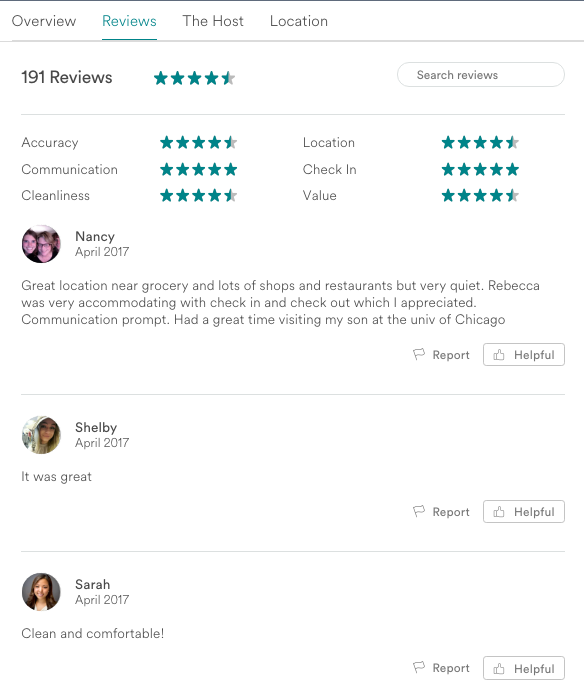
\includegraphics[width=.8\textwidth]{figures/sample3-reviews}
\caption{Sample review information}
\end{figure}
\begin{figure}\centering
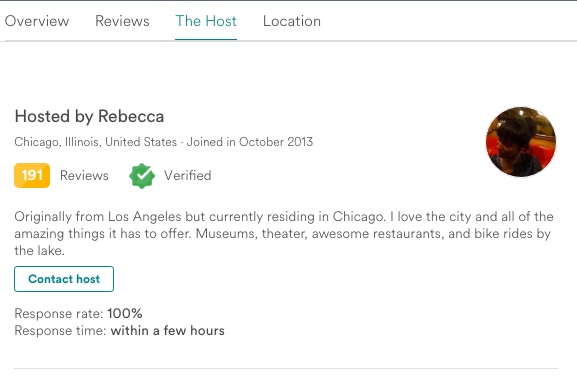
\includegraphics[width=.9\textwidth]{figures/sample4-host}
\caption[Sample host information]{Sample host information available.}
\end{figure}
\begin{figure}\centering
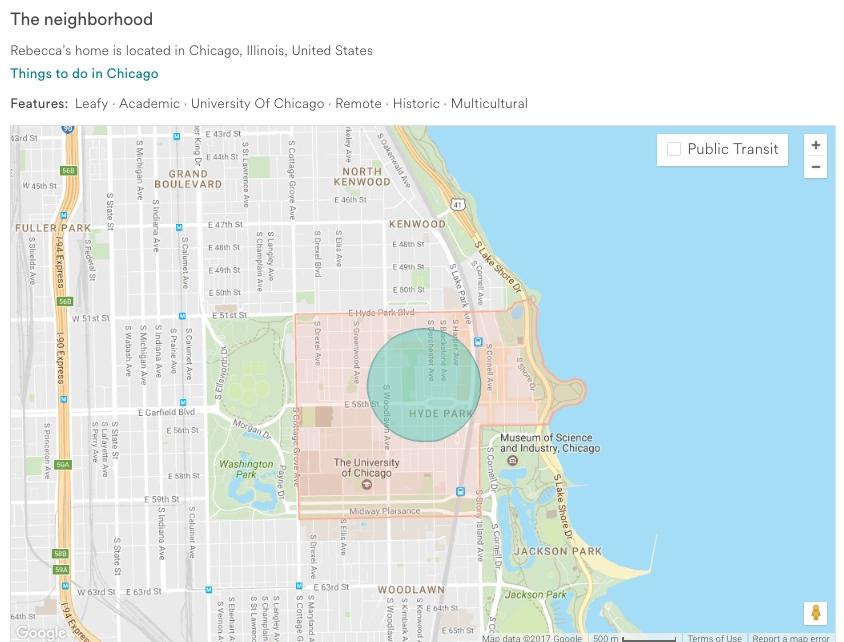
\includegraphics[width=.8\textwidth]{figures/sample5-location}
\caption{Sample location information}
\end{figure}
\begin{figure}\centering
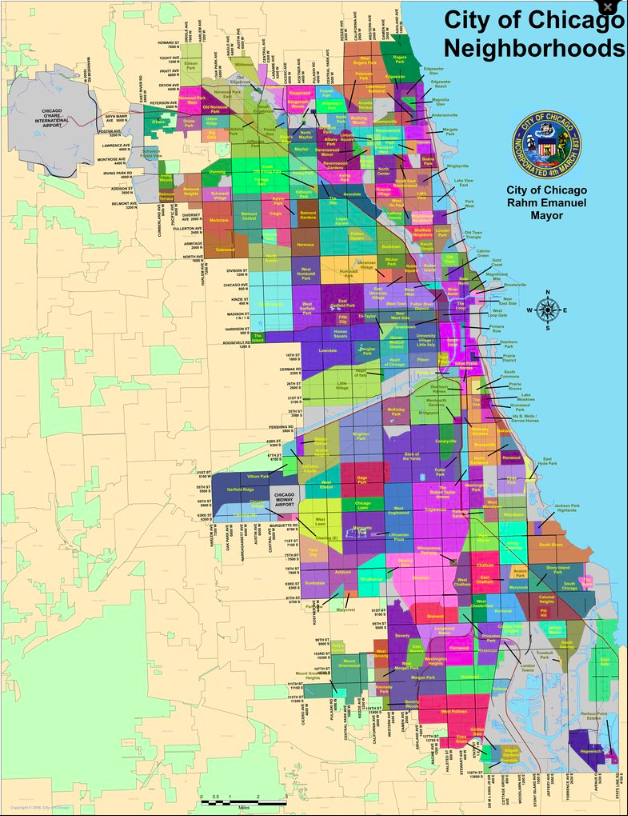
\includegraphics[width=.8\textwidth]{figures/chicago_city_neighborhoods}
\caption[City of Chicago neighborhoods]{City of Chicago neighborhoods, showing level of granularity of neighborhood controls}
\end{figure}




\newpage


\begin{comment} 
In this section, I consider alternative explanations for the price differences I found between minority and white hosts. In particular, I examine three relevant mechanisms that are not discrimination that could explain my results. I will then argue that these mechanisms would be insufficient in doing so. 

\textbf{2. Price observed during the scrape is not the price normally set by hosts or observed by guests}

The prices I used in my data analysis were prices from one particular day in 2015-2016. I ran my regressions on the assumption that this is the price that hosts set and that guests observe that drives guest booking decisions and host revenue outcomes. However, imagine that for one day, all of the white people on Airbnb raise their prices. That day, the scrape happens to take place, and the next day, the prices of White hosts all go back down. Then, the price that I observed in my data for White hosts would be high even though it doesn't incorporate real demand differences between races nor is tied to listing characteristics or host quality. While this may seem like an unlikely scenario, price hikes for the weekend or for holidays like July 4th or New Year's may give rise to a similar situation if black hosts change their prices differently than White hosts. 

TO-DO - Check price time series data to prove that prices don't move around that much during the month/year. 

\textbf{3. Data clean-up disproportionately dropped lower-priced listings of White hosts or higher-priced listings of minority hosts}

During my analysis, I left out hosts that had no profile picture. If hosts are aware of the potential effects of discrimination, minority hosts might be less likely to include a profile picture. If minority hosts who own higher-priced listings dropped out of the data set in this way, my coefficients might be biased downward because the sample doesn't include the higher-priced listings owned by minority hosts. A similar thing could have happened when I restricted my data set to listings with a price per night of less than \$800, and to listings owned by hosts who owned fewer than 20 listings total. If those hosts who owned a lot of listings or charged wildly high prices per night were disproportionately black, Hispanic, or Asian, I'd see a similar downward bias on my coefficients.

TO-DO - Examine who I am dropping when I do data-clean up. 

************Garbage
After controlling for listing characteristics, host characteristics, and the neighborhood location of the Airbnb, and time on the market, I find that all host categories, but especially black male hosts, white female hosts, black female hosts, and Asian female hosts, for whom the result is statistically significant at at least the p < .01 level, earn approximately \$200 less during the course of their listing than white male hosts.  will earn \$190 - \$284 less revenue from their Airbnb over the course of the posting relative to their white male peers. The effect is statistically significant at the p < .001 level for white female and black female hosts, and significant at the p < .01 level for black male hosts and Asian female hosts. While there is a large downward effect on revenue for Hispanic male, Hispanic female, and Asian male hosts, it does not persist after controlling for listing and host characteristics. Contrary to what one would expect from discrimination literature, out of the groups for whom I could measure discrimination, black male fared the least poorly, earning \$190 less than white male hosts over the course of their listing?s lifetime. Women as a whole, regardless of race, do worse than black men. Asian women earn \$232.6 less in revenue and white women earn \$272 less in revenue than white male peers. Black women hosts fare the worst out of any of the groups considered, earning \$283.6 less than white men over the course of their Airbnb listing. 

white male reviewers gave lower reviews only to Asian female, with a .074-unit decrease relative to white male hosts. Black male guests gave white female hosts .207 units, two white male hosts .624 lower, Asian men .517 units higher quality reviews than they gave white men. White females gave lower quality reviews only to Asian women at a rate of .099 units less. Black female reviewers gave Airbnbs owned by two black women an entire valence point, 1.005 units better reviews than white male hosts, but rated Hispanic women .647 units lower. Asian females rated Black male hosts .358 units worse than white male hosts. 


TO-DO: Add Levitt and Fryer? Black names paper
List (2004) found a similar result at baseball card shows, with Black sellers getting offer 3-30\% worse than White sellers. 

Becker explains, ``If someone has a `taste for discrimination', he must act as if he were willing to forfeit income in order to avoid certain transactions; it is necessary to be aware of the emphasis on the words `as if'" (Becker 16).While market discrimination harms the discriminated group because it lowers their wages, taste discrimination can also harm the person discriminating, since they might now be paying more for the same good or service - whether in opportunity cost or price -  because they prefer not to interact with the discriminated group. 
Another type of discrimination laid out by Becker is taste discrimination, in which people ``prefer" not to interact with certain groups. This type of taste discrimination that is based on a general dislike could show up in the reviews that are left on host profiles. If a guest stays with a host against whom they are prejudiced, they may leave a worse review or rating, a shorter review, or no review at all, than a comparable stay with a white host. 

********former introduction

When Dyne Suh was minutes away from arriving at the Airbnb she had booked for a weekend getaway, she received a cancellation notice from the host. Left stranded in a snowstorm, Suh offered to pay extra for her stay. The host, through a series of racist messages on the Airbnb app, revealed that she had cancelled because Suh appeared Asian.\cite{diane}  

This example from February 2017 is an extreme case of overt racism, and ended in Airbnb permanently banning the host from the platform. Yet, over the past several years, users have reported more subtle discrimination on Airbnb through social media stories of hosts cancelling or rejecting guests.\cite{nyt1} After being under fire for most of the year, Airbnb updated its Discrimination Policy in September 2016, increasing instant bookings (the opportunity for guests to book without waiting for host approval) and making host profile pictures smaller.\cite{nyt2} 

Sharing economies platforms create a particularly complex environment for regulating discrimination. On the one hand, agents are constrained by certain features of the user interface - if Airbnb never provided guests with a picture or the name of the host, there would be little opportunity to discriminate. On the other hand, users ultimately have nearly full control of the transactions they engage in. For example, drivers on Uber can choose not to accept certain trips or turn the app on or off at their convenience. 

However, these stories of discrimination against \textit{guests} provide only anecdotal evidence for the larger problem of discrimination in the Airbnb market. The problem of discrimination against \textit{hosts} is not publicized, even though it just as important because it affects the prices, revenues, and sometimes livelihoods of thousands of Airbnb hosts. 
\iffalse %comments out entire section of text
\begin{quotation}
``Suppose there are two groups, designated by $W$ and $N$, with members of $W$ being perfect substitutes in production for members of $N$. In the absence of discrimination and nepotism and if the labor market were perfectly competitive, the equilibrium wage rate of $W$ would equal that of $N$. Discrimination could cause these wage rates to differ; the market discrimination coefficient between $W$ and $N$ [...] is defined as the proportional difference between these wage rates" \end{quotation}
\fi
\end{comment}


\end{document}  